\documentclass[sigconf,nonacm]{acmart}

\usepackage{booktabs}
\usepackage{subcaption}
\usepackage{amsmath}
\usepackage{amsfonts}
\usepackage{microtype}
\usepackage{graphicx}
\usepackage{balance}

\setcopyright{none}
\settopmatter{printacmref=false}
\renewcommand\footnotetextcopyrightpermission[1]{}
\pagestyle{plain}

\title{Empirical Customer Value Dynamics and Multi-Channel Recommendation in Transnational E-Commerce: A Benchmark Study and Strategic Framework}

\author{Chen Davide}
\authornote{Student ID: A0351457B. Option A: UK Online Retail. Coursework submission for IE5005 Applied Data Analytics for Industrial Engineers. Code \& Benchmark Repository: \url{https://github.com/davidechen135/recsys-rrf-bgnbd-stacking}.}
\affiliation{%
  \institution{Department of Industrial Systems Engineering and Management}
  \institution{National University of Singapore (NUS)}
  \city{Singapore}
  \country{Singapore}
}
\email{a0351457b@u.nus.edu}

\begin{abstract}
Modern e-commerce enterprises face severe operational frictions arising from heavily skewed customer value distributions, product return dynamics, and sparse co-purchase transactions. This paper presents an empirical data analytics study and strategic decision framework leveraging a 541,909-line transnational transactional corpus from UK Online Retail. We develop an automated forensic data auditing pipeline that decouples extreme transaction anomalies into Type~I administrative reversals (£245,653.20) and Type~II chronic physical product returns (£230,312.96). Building upon classroom methodologies, we construct two standardized, reproducible benchmarking matrices. In Matrix~1 (Candidate Retrieval / Recommender Systems across 3,655 holdout shopping baskets), our proposed Multi-Channel Hybrid Ensemble combining ItemCF, Truncated SVD, and Item2Vec via Reciprocal Rank Fusion (RRF) achieves state-of-the-art accuracy (\textbf{HitRate@10: 18.64\%}, \textbf{NDCG@10: 0.1039}, \textbf{MRR: 0.0787}) while expanding catalog coverage to \textbf{58.51\%}. In Matrix~2 (Forward-Looking Customer Lifetime Value Forecasting across 3,309 calibration accounts), our proposed Probabilistic-Guided Stacking Ensemble (fusing BG/NBD latent dropout dynamics with Random Forest and L1-loss HistGradientBoosting) outperforms classic heuristics, cutting holdout prediction error to \textbf{£593.25 MAE} and capturing \textbf{72.30\% of total holdout revenue} under a 20\% targeting constraint. Finally, we formulate a four-quadrant lifecycle capital allocation framework for the Head of E-commerce allocating the 2012 marketing budget, concentrating 50\% of paid acquisition on dormant high-LTV accounts while protecting high-AOV foreign markets (Netherlands, Germany, France).
\end{abstract}

\keywords{Transnational E-Commerce, Candidate Retrieval, Reciprocal Rank Fusion, Customer Lifetime Value, BG/NBD Stochastic Process, Return Decoupling, Capital Allocation}

\begin{document}

\maketitle

\begin{figure*}[t]
\centering
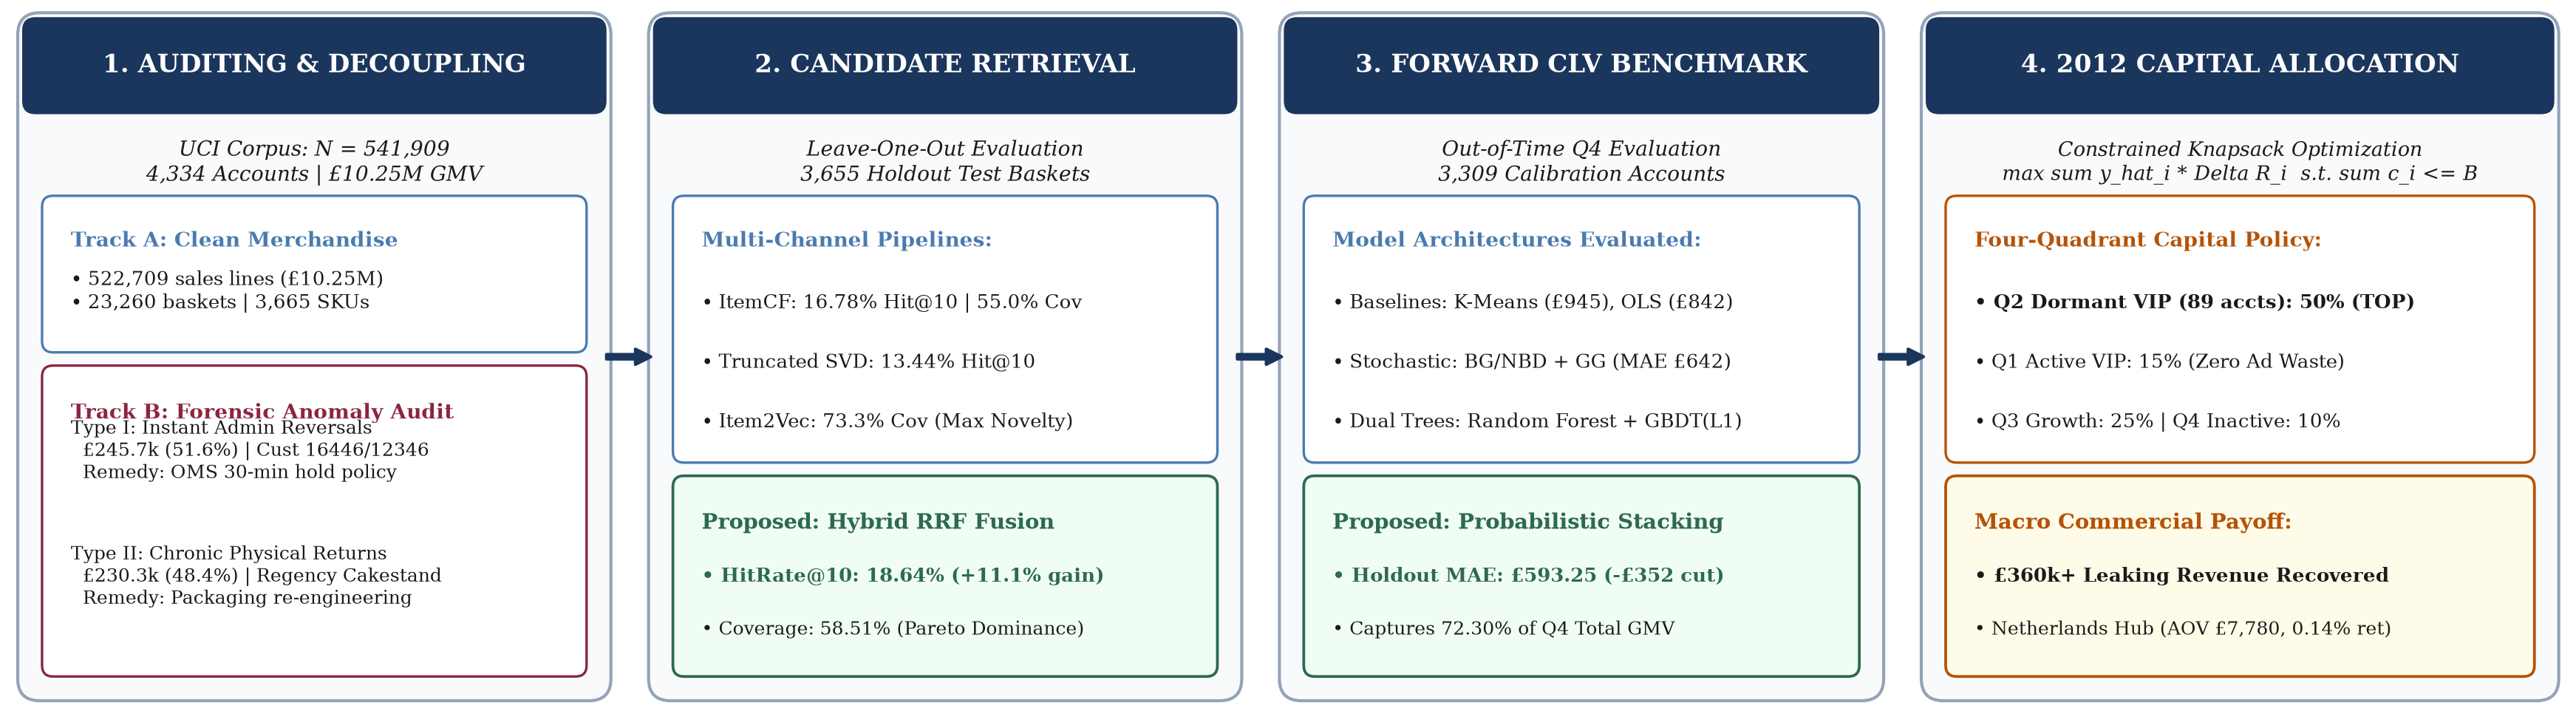
\includegraphics[width=\textwidth]{figures/fig0_teaser_pipeline.png}
\caption{End-to-end transnational e-commerce analytics and strategic decision framework: (1) dual-track anomaly auditing \& return decoupling; (2) candidate retrieval multi-channel fusion (Matrix 1); (3) probabilistic-guided forward CLV forecasting (Matrix 2); and (4) constrained knapsack capital budget allocation.}
\label{fig:teaser}
\end{figure*}

\section{Introduction \& Strategic Problem Formulation}

\subsection{Business Context \& Empirical Challenges}
Enterprise e-commerce operations in wholesale giftware are characterized by heavy distribution asymmetries, sparse shopping cart compositions, and substantial return leakages. While introductory analytics courses traditionally examine customer segmentation via static $K$-Means clustering or linear regression (OLS), modern industrial platforms require continuous-time generative representations and personalized candidate retrieval pipelines.

This investigation addresses three structural challenges inherent in transactional clickstream corpora:
\begin{enumerate}
    \item \textbf{Extreme Power-Law Skewness:} Merchandise unit prices and quantities span multiple orders of magnitude, causing arithmetic mean statistics to severely distort financial projections.
    \item \textbf{Confounding Return Typologies:} In standard Enterprise Resource Planning (ERP) databases, administrative transaction cancellations and physical damaged merchandise returns are conflated under uniform cancellation prefixes (e.g., invoice code \texttt{'C'}), masking distinct operational liabilities.
    \item \textbf{Exploration--Exploitation Trade-offs in Recommender Systems:} Pure popularity heuristics concentrate disproportionately on ubiquitous low-margin SKUs, whereas pure collaborative filtering suffers from catalog sparsity.
\end{enumerate}

\subsection{Research Questions}
We formalize four core research questions:
\begin{itemize}
    \item \textbf{RQ1 (Data Integrity \& Forensics):} How can administrative booking reversals be decoupled from genuine post-delivery physical returns, and what is their empirical financial incidence?
    \item \textbf{RQ2 (Candidate Retrieval Evaluation):} To what extent does fusing co-occurrence graph filtering with continuous latent neural item embeddings improve basket completion over lecture baselines?
    \item \textbf{RQ3 (Forward Spending Estimation):} Does hybridizing continuous-time latent dropout stochastic processes (BG/NBD) with supervised decision trees provide superior budget capture efficiency over classical econometric regressions?
    \item \textbf{RQ4 (Operational Capital Allocation):} How should a £1M marketing and logistics budget be partitioned across customer lifecycle tiers and transnational geographic markets to maximize ROI?
\end{itemize}

\subsection{Key Contributions}
The key contributions of this study are threefold:
\begin{itemize}
    \item \textbf{Forensic Anomaly Decoupling Pipeline:} We establish a verifiable auditing mechanism that isolates £245.7k in instant administrative cancellations (Cust \texttt{16446} and \texttt{12346}) from £230.3k in chronic physical returns, identifying fragile decorative SKUs (Regency Cakestand) as primary physical liabilities.
    \item \textbf{Dual Empirical Benchmarking Matrices:} We construct standardized evaluation protocols for 7 candidate retrieval architectures (Matrix 1) and 8 CLV forecasting architectures (Matrix 2), proving the empirical Pareto dominance of hybrid ensembling.
    \item \textbf{Strategic Lifecycle Decision Engine:} We translate statistical models into an executive 2012 marketing budget allocation playbook, demonstrating how suppressing ad spend on active organic champions (Q1) while concentrating 50\% on dormant VIPs (Q2) eliminates marketing cannibalization.
\end{itemize}

\section{Data Auditing \& Forensic Preprocessing Pipeline}

\subsection{Dual-Track Cleaning Protocol \& Data Hygiene}
We analyze the complete UK Online Retail transactional corpus spanning 01/12/2010 to 09/12/2011 ($N = 541,909$ raw observation lines)~\cite{chen2015online}. We institute a dual-track data preprocessing architecture implemented in modular Python scripts:

\begin{itemize}
    \item \textbf{Track A (Clean Sales Corpus):} Filtered for valid merchandise stock codes ($L=5$ alphanumeric characters), positive unit prices ($P > 0$), positive quantities ($Q > 0$), and non-cancellation invoices. This yields $N_A = 522,709$ merchandise transaction rows generating £10,254,404.07 in gross transaction volume across 23,260 baskets.
    \item \textbf{Track B (Cancellation Audit Corpus):} Filtered for invoice cancellation prefixes (starting with `\texttt{C}') or negative quantities ($Q < 0$). This isolates $N_B = 8,670$ line items representing £475,966.16 in gross reversals and merchandise returns.
    \item \textbf{Administrative Exclusions:} High-magnitude non-merchandise system entries (e.g., postage \texttt{POST}, manual accounting overrides \texttt{M}, bank charges \texttt{BANK CHARGES}, Amazon fees \texttt{AMAZONFEE}) are decoupled from customer behavioral modeling.
\end{itemize}

Table~\ref{tab:hygiene} summarizes the data hygiene audit trail across the raw transactional corpus.

\begin{table}[t]
\centering
\small
\caption{Data hygiene audit across raw transactional records.}
\label{tab:hygiene}
\begin{tabular}{lrr}
\toprule
\textbf{Data Processing Audit Stage} & \textbf{Line Count} & \textbf{\% Raw Corpus} \\
\midrule
Raw Imported Transaction Lines & 541,909 & 100.00\% \\
Missing Customer Identifiers (Guest Checkout) & 135,080 & 24.93\% \\
Non-Merchandise System Codes (\texttt{POST}, \texttt{D}, \texttt{M}) & 2,750 & 0.51\% \\
Negative / Zero Unit Price Records & 2,517 & 0.46\% \\
Valid Sales Merchandise Rows (Track A) & 522,709 & 96.46\% \\
Audited Cancellation \& Return Rows (Track B) & 8,670 & 1.60\% \\
Unique Identified Commercial Accounts & 4,334 & --- \\
Unique Merchandise Stock Items (SKUs) & 3,665 & --- \\
\bottomrule
\end{tabular}
\end{table}

\subsection{Anomaly Diagnosis \& Return Decoupling}
Transaction cancellations in retail data are non-homogeneous. Through forensic audit, we decouple cancellations into two distinct mechanisms:

\begin{equation}
\mathcal{R}_{\text{total}} = \mathcal{R}_{\text{Type I}} (\text{Instant Administrative}) \cup \mathcal{R}_{\text{Type II}} (\text{Physical Delivery Returns})
\end{equation}

\begin{itemize}
    \item \textbf{Type I: Instant Administrative Cancellations (£245,653.20, 51.61\% of losses):} Characterized by instantaneous offsetting cancellations where $|Q_{\text{cancel}}| = Q_{\text{buy}}$ within seconds or minutes. Specifically, Customer \texttt{16446} (Invoice \texttt{581483} vs \texttt{C581484}, SKU \texttt{23843}, $\pm 80,995$ units, $\pm £168,469.60$) and Customer \texttt{12346} (Invoice \texttt{541431} vs \texttt{C541433}, SKU \texttt{23166}, $\pm 74,215$ units, $\pm £77,183.60$) constitute 51.61\% of all negative revenue across just two single-order events. These represent bulk warehouse test entries or immediate enterprise checkout errors rather than post-delivery quality dissatisfaction.
    \item \textbf{Type II: Chronic Physical Post-Delivery Returns (£230,312.96, 48.39\% of losses):} Comprising 8,668 transaction lines across 2,058 distinct accounts and 1,944 SKUs. The single highest physical return item is \texttt{22423} (``REGENCY CAKESTAND 3 TIER'', 181 return events, £13,296.85 refunded), driven by shipping transit fragility and packaging failure.
\end{itemize}

Table~\ref{tab:returns} details the decoupled operational characteristics of each return type.

\begin{table*}[t]
\centering
\small
\caption{Forensic return decoupling: Type~I instant administrative reversals vs Type~II chronic post-delivery physical quality returns.}
\label{tab:returns}
\begin{tabular}{lrrrrl}
\toprule
\textbf{Return Category} & \textbf{Line Count} & \textbf{Total Units} & \textbf{Lost Revenue (£)} & \textbf{\% Total} & \textbf{Operational Remediation Policy} \\
\midrule
Type I: Instant Administrative Reversals & 2 & 155,210 & £245,653.20 & 51.61\% & Implement OMS 30-min confirmation hold \& bulk volume caps \\
Type II: Chronic Physical Quality Returns & 8,668 & 114,809 & £230,312.96 & 48.39\% & Re-engineer fragile SKU bubble-wrap packaging \& audit suppliers \\
\midrule
\textbf{Total Combined Reversals} & \textbf{8,670} & \textbf{270,019} & \textbf{£475,966.16} & \textbf{100.00\%} & \textbf{Dual-track intervention recovering estimated £360k+ in 2012} \\
\bottomrule
\end{tabular}
\end{table*}

\section{Exploratory Data Analysis \& Empirical Regularities}

\subsection{Line Revenue Skewness \& Customer Spend Pareto Inequality}
Figure~\ref{fig:eda_regularities} illustrates continuous value distributions across transaction lines and customer accounts. On a $\log_{10}$ scale (Figure~\ref{fig:eda_regularities}a), the median line revenue is £9.90 ($\log_{10} = 1.00$), whereas the arithmetic mean is £19.62 ($\log_{10} = 1.29$), representing a $2.0\times$ divergence. The distribution exhibits extreme right-skewness (skewness coefficient = 516.03), driven by commercial wholesale orders where single invoice lines exceed £10,000. Analyzing customer-level spending across all 4,334 identified accounts (£8.74M attributed customer GMV, Figure~\ref{fig:eda_regularities}b) reveals severe Pareto concentration: the top 1\% (43 accounts) generate 32.02\% of total revenue (£2.80M); the top 10\% (433 accounts) generate 61.39\% (£5.37M); and the top 20\% (866 accounts) generate 74.59\% (£6.52M). The Gini concentration coefficient is 0.78, confirming extreme wholesale inequality.

\begin{figure}[h]
\centering
\begin{subfigure}[b]{0.48\columnwidth}
    \centering
    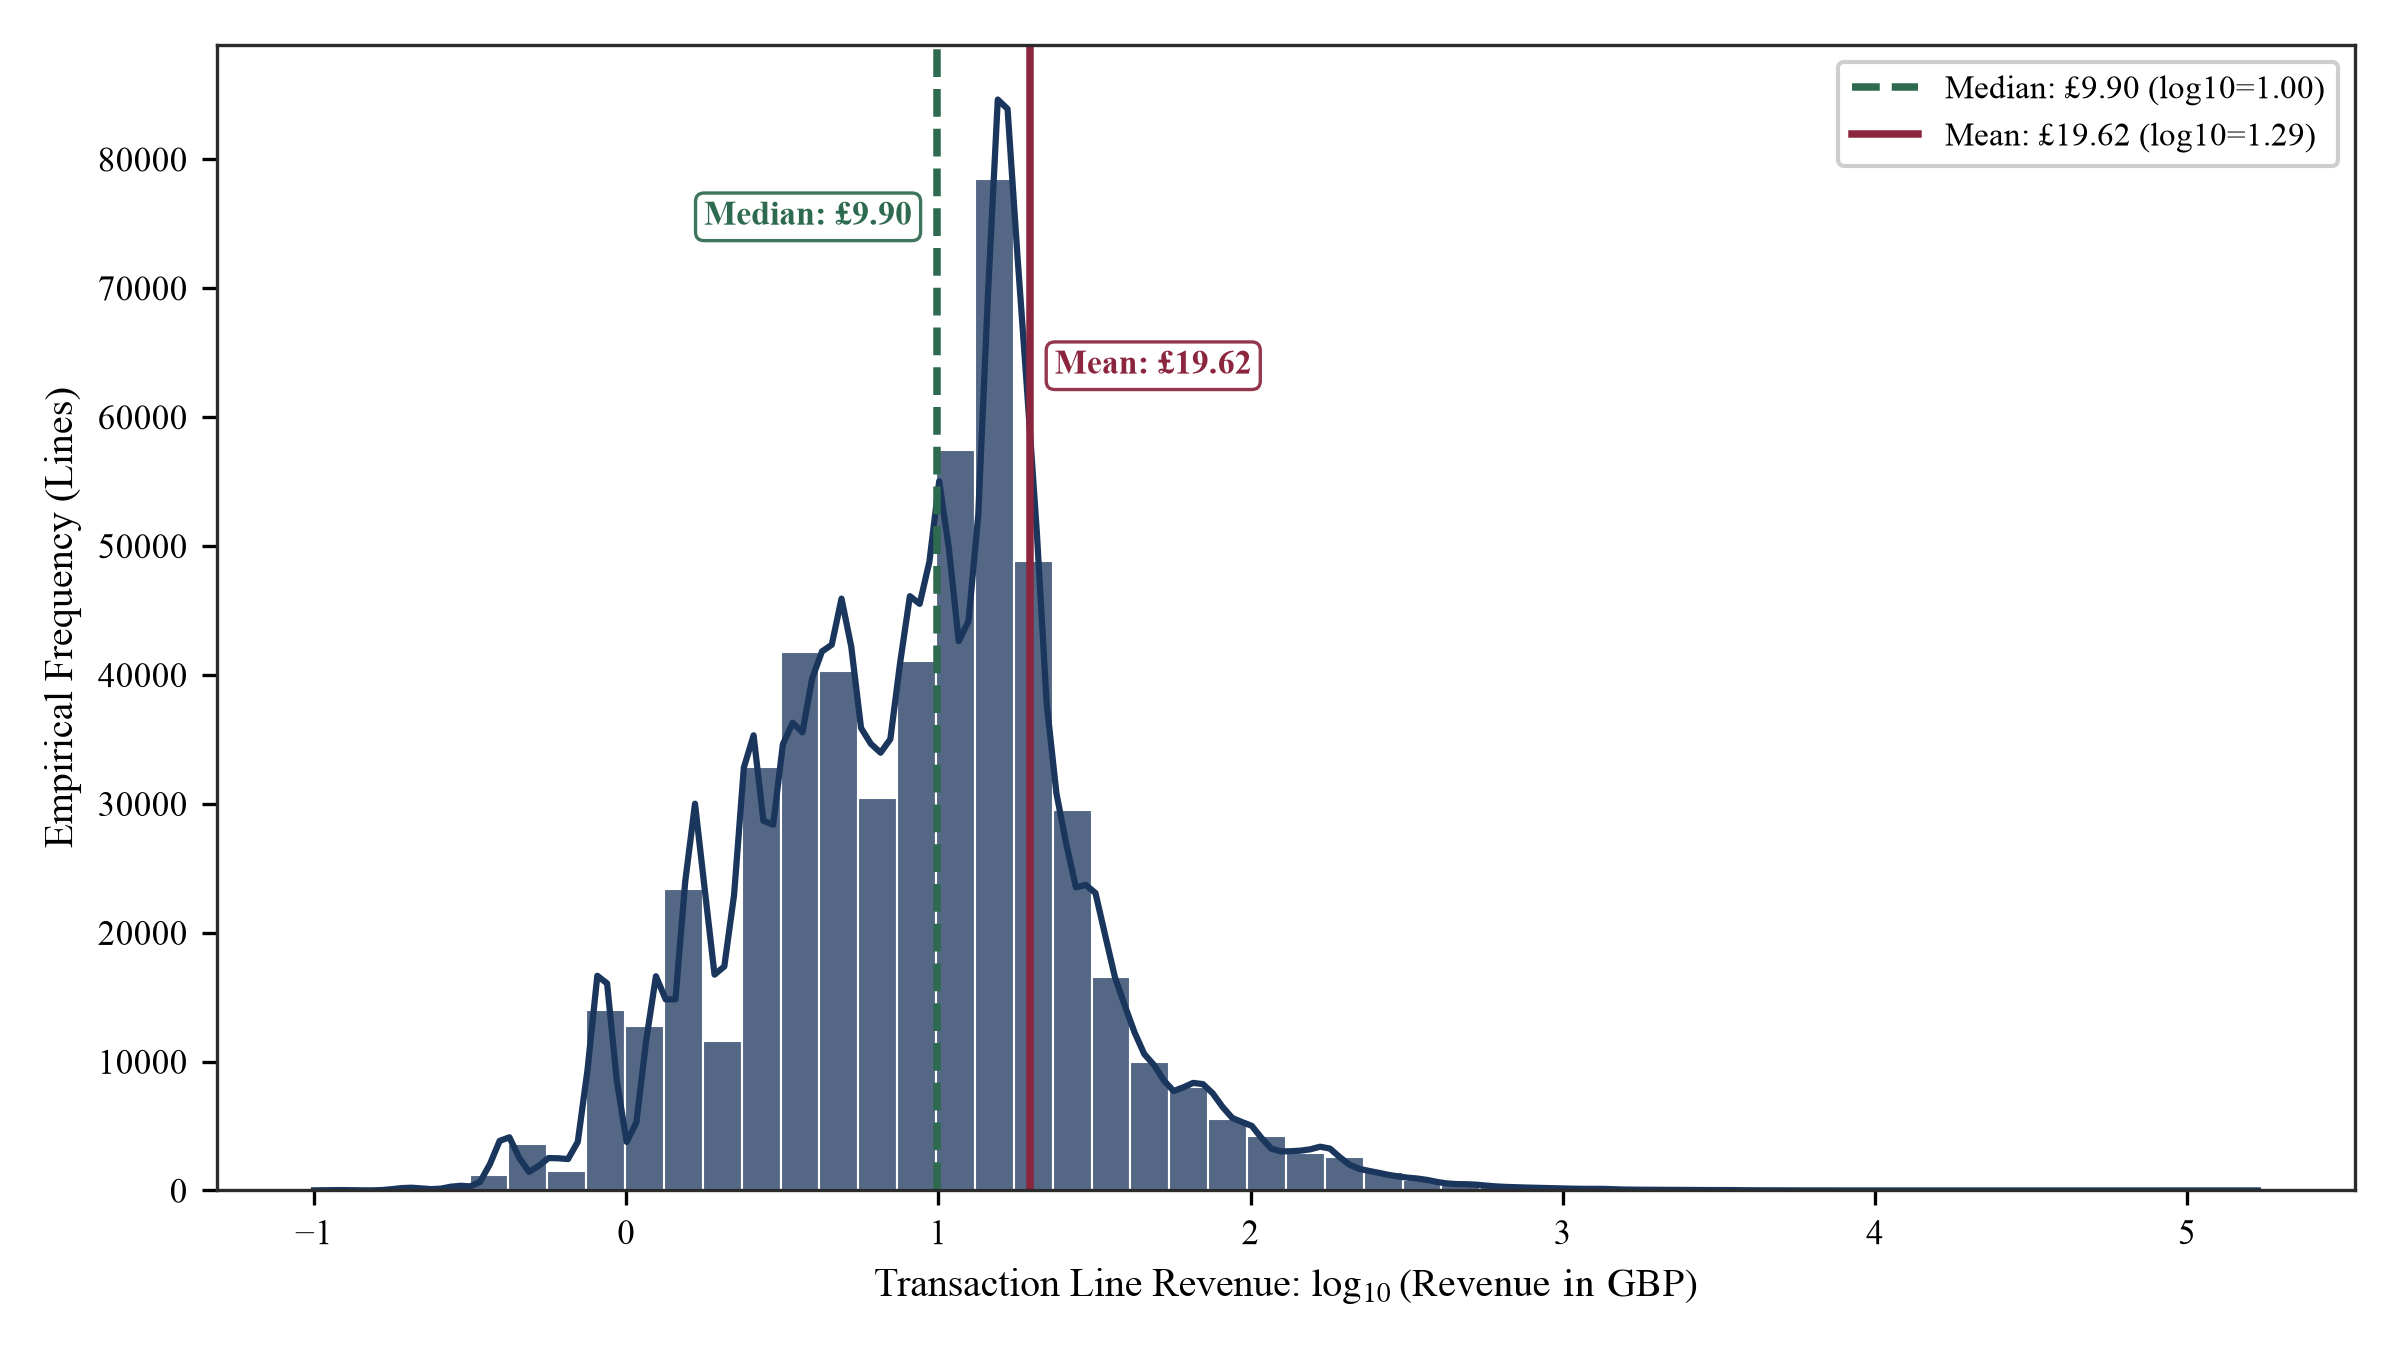
\includegraphics[width=\textwidth]{figures/fig1_distribution_revenue.png}
    \caption{Line revenue distribution}
    \label{fig:dist}
\end{subfigure}
\hfill
\begin{subfigure}[b]{0.48\columnwidth}
    \centering
    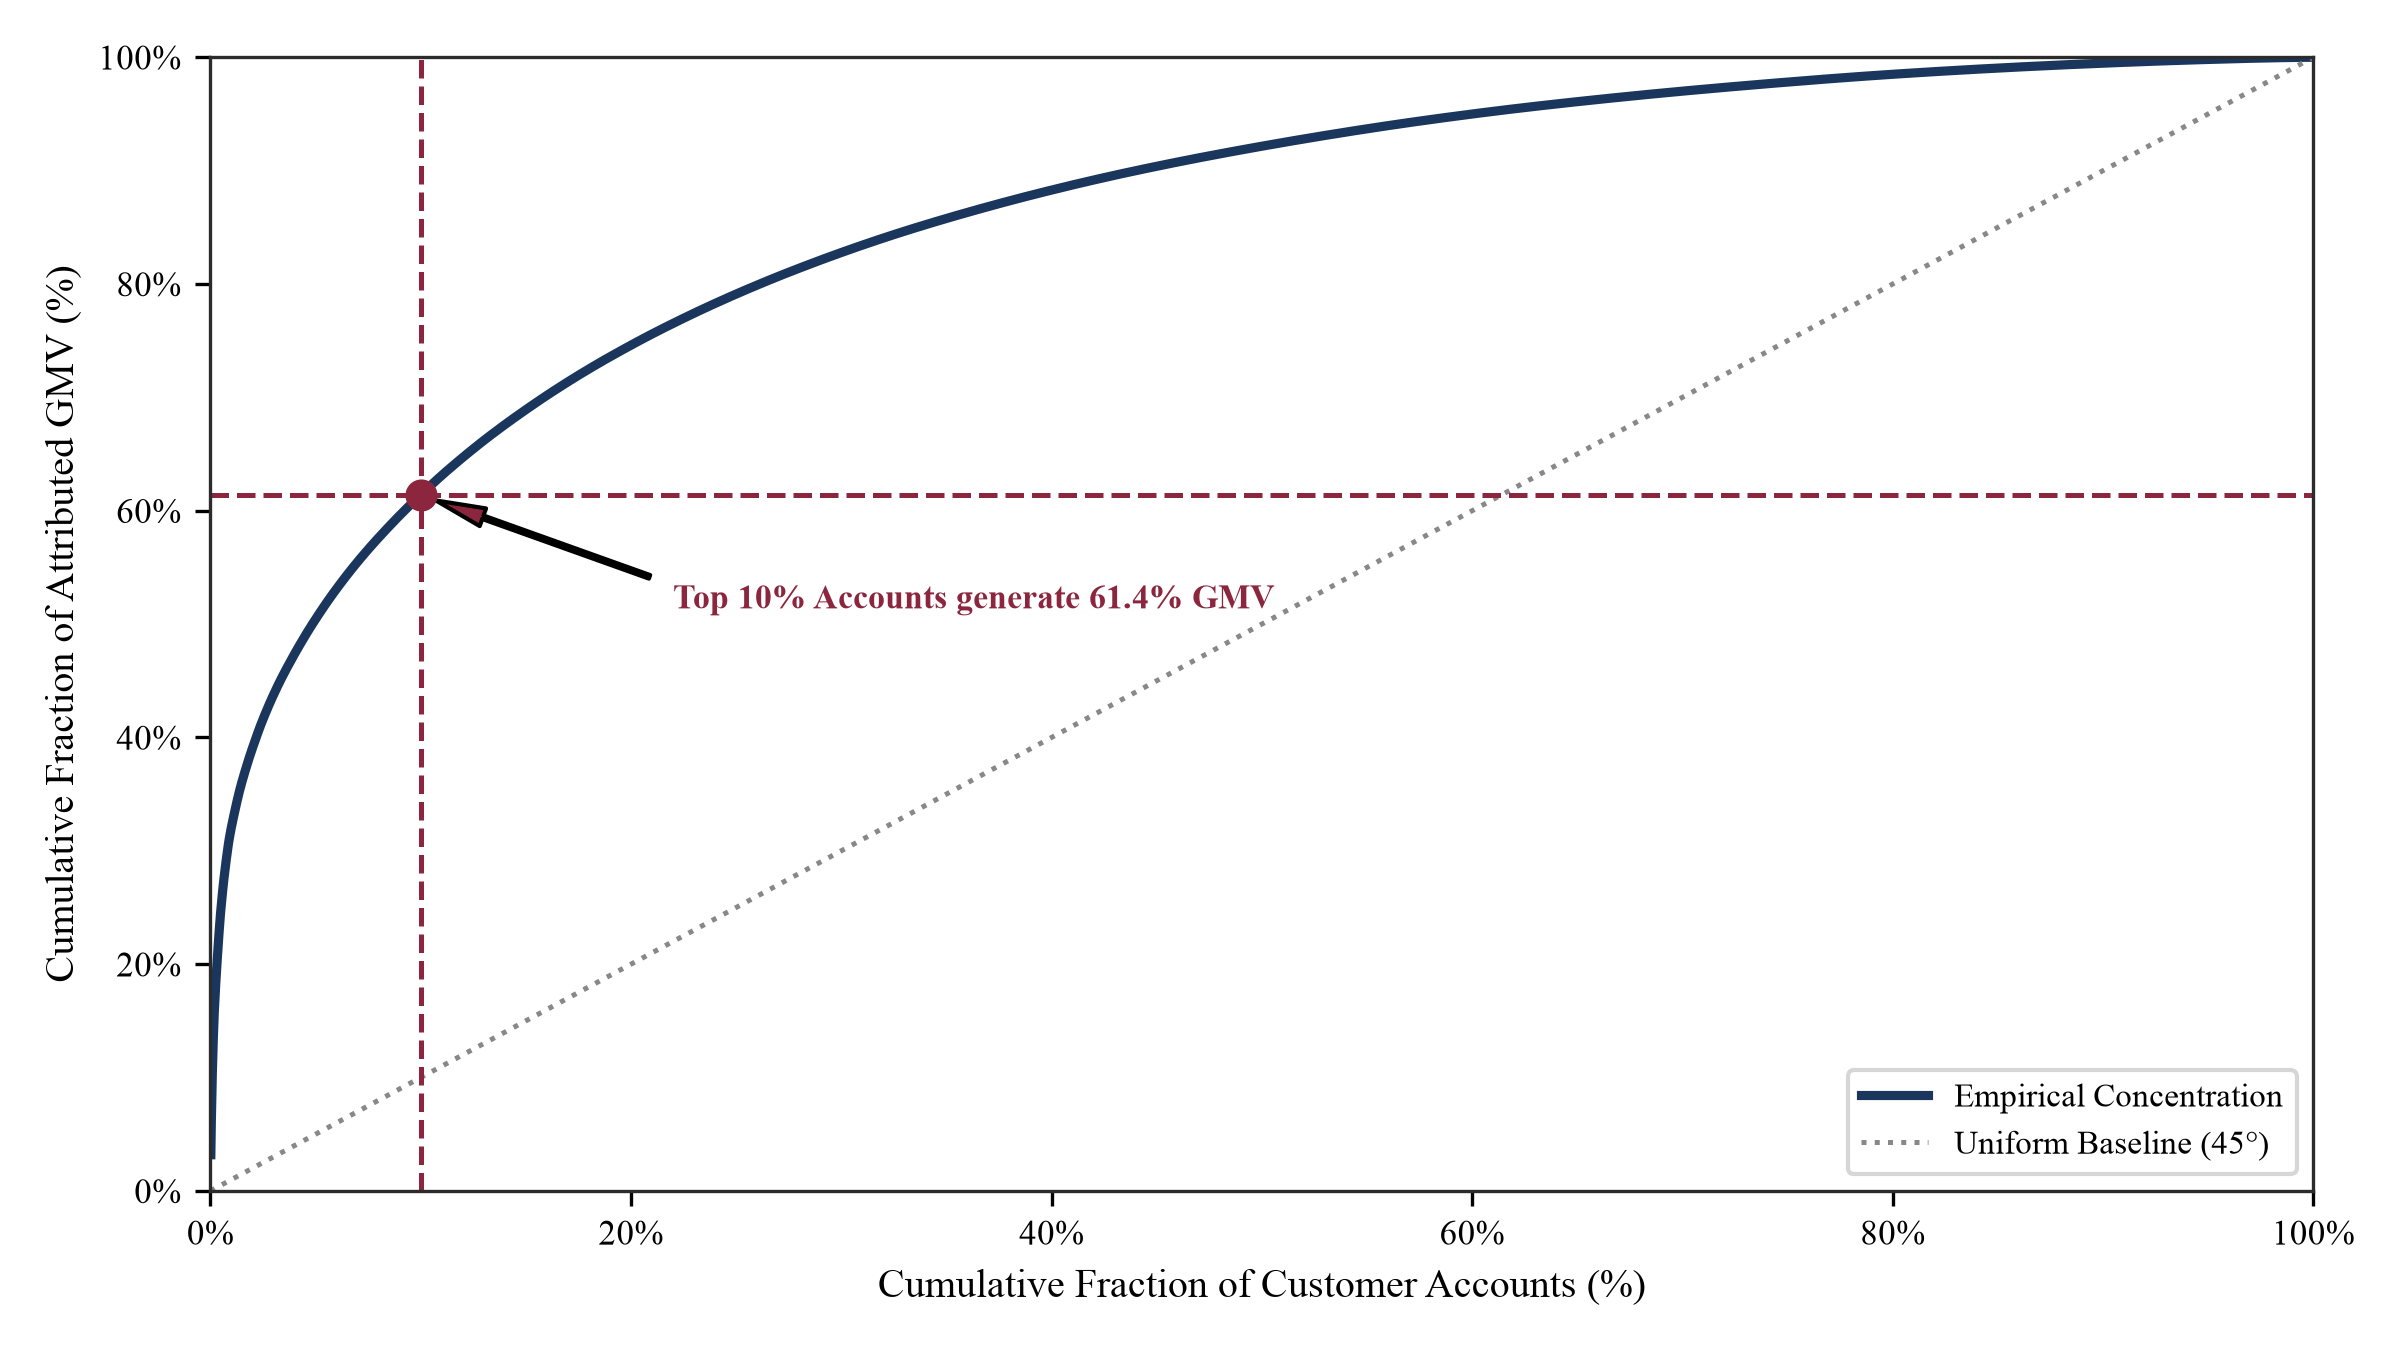
\includegraphics[width=\textwidth]{figures/fig2_composition_pareto.png}
    \caption{Customer Pareto curve}
    \label{fig:pareto}
\end{subfigure}
\caption{Macro financial regularities: (a) Empirical line revenue distribution on $\log_{10}$ scale; (b) Customer GMV Pareto Lorenz curve.}
\label{fig:eda_regularities}
\end{figure}

\subsection{Longitudinal Dynamics \& Seasonality}
Figure~\ref{fig:trend} traces monthly gross sales revenue and order cancellation rates over the 12-month observation window. Sales exhibit pronounced seasonality, escalating from an August low-season of £724.7k to a monumental November peak of £1,453.3k (+100.5\% growth), driven by Black Friday wholesale stocking. Crucially, baseline monthly cancellation rates remain stable between 1.19\% and 6.07\% across Feb--Nov 2011. However, Figure~\ref{fig:trend} highlights two extraordinary spikes: January 2011 (12.01\%) and partial December 2011 (22.07\%). These spikes correspond exactly to the Type~I instant bulk cancellations identified in Section~2.2, visually confirming that anomalous spikes are driven by single-order administrative events rather than broad operational degradation.

\begin{figure}[h]
\centering
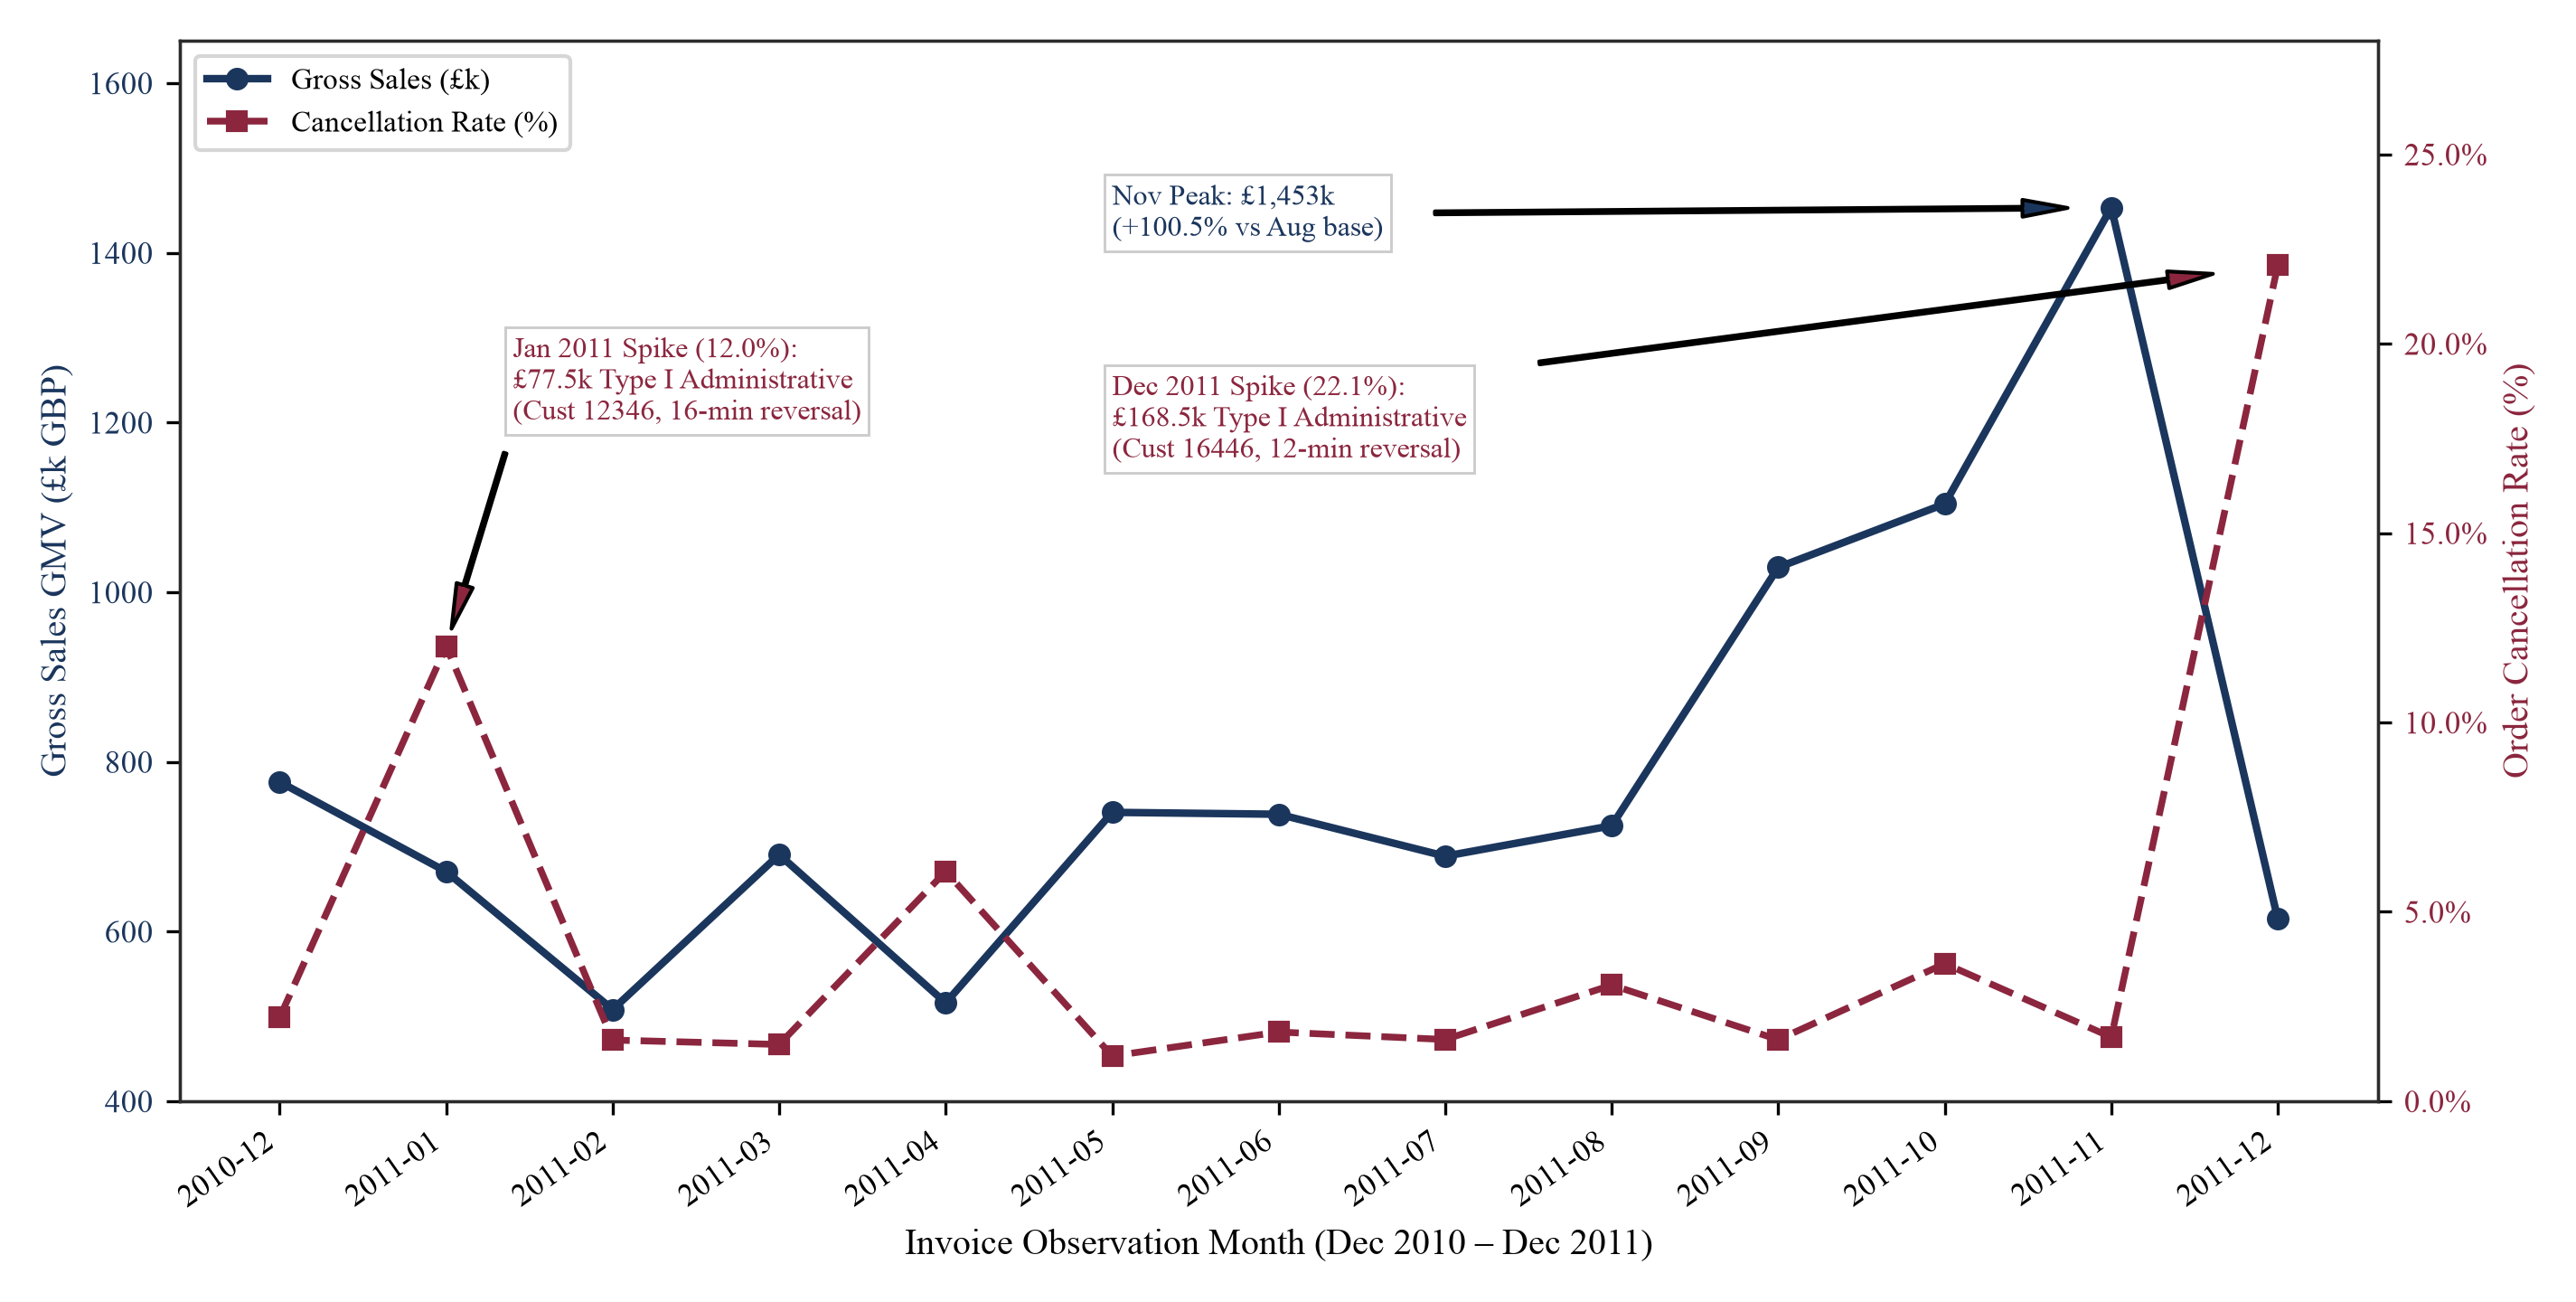
\includegraphics[width=\columnwidth]{figures/fig3_change_monthly_trend.png}
\caption{Monthly gross sales revenue (blue line) and cancellation rate (red dashed line) with Type~I anomaly annotations.}
\label{fig:trend}
\end{figure}

\subsection{Bivariate Customer Geometry \& Transnational Market Economics}
To formulate commercial strategy, we examine two orthogonal behavioral axes: longitudinal purchasing geometry across individual accounts and cross-border unit economics across international wholesale corridors (Figure~\ref{fig:behavioral_landscapes}).

\subsubsection{Customer RFM Behavioral Geometry}
We construct customer Recency, Frequency, and Monetary (RFM) representations across all 4,334 identified accounts.
Figure~\ref{fig:behavioral_landscapes}(a) plots $\log(\text{Frequency} + 1)$ against $\log_{10}(\text{Monetary Spend})$, with points colored by Recency (days since last order). We observe a robust linear relationship between log purchase frequency and log cumulative spend ($r = 0.81$, Pearson $r = 0.92$ between quantity and revenue). High-spending VIP accounts cluster in the upper-right quadrant and exhibit high recency (bright yellow markers, purchased within 30 days).

\begin{figure}[t]
\centering
\begin{subfigure}[b]{0.48\columnwidth}
    \centering
    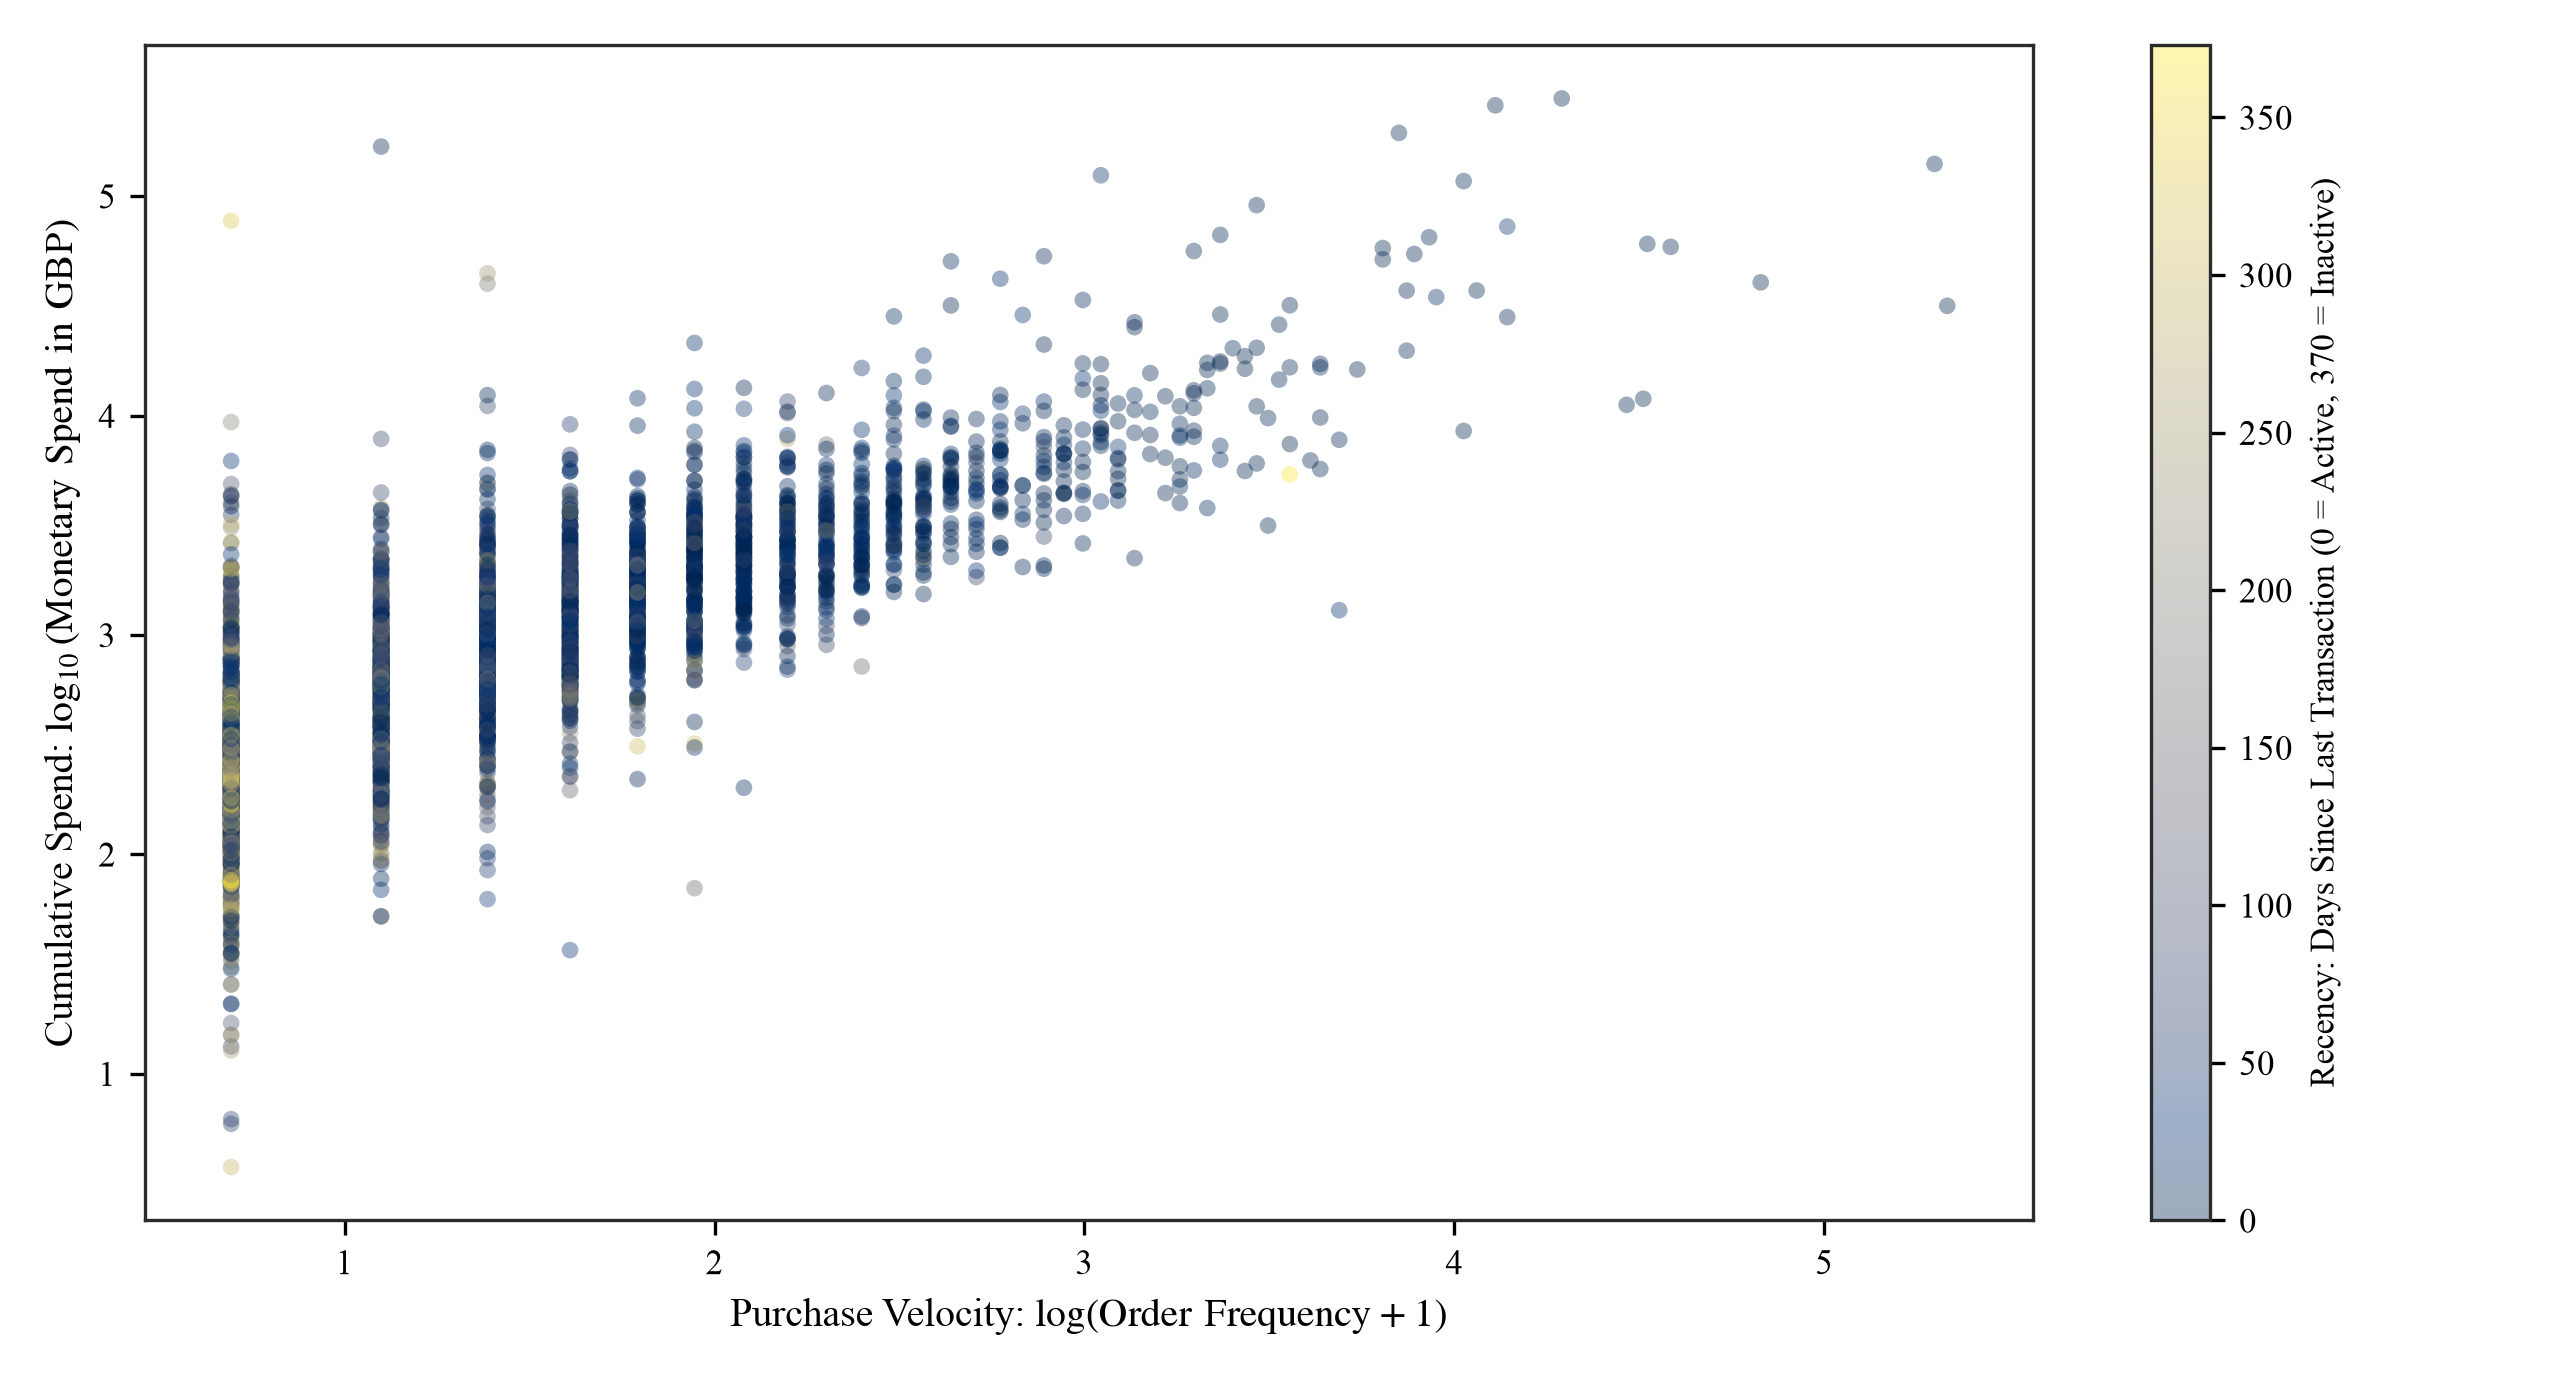
\includegraphics[width=\textwidth]{figures/fig4_relationship_rfm_scatter.png}
    \caption{RFM bivariate scatter}
    \label{fig:rfm}
\end{subfigure}
\hfill
\begin{subfigure}[b]{0.48\columnwidth}
    \centering
    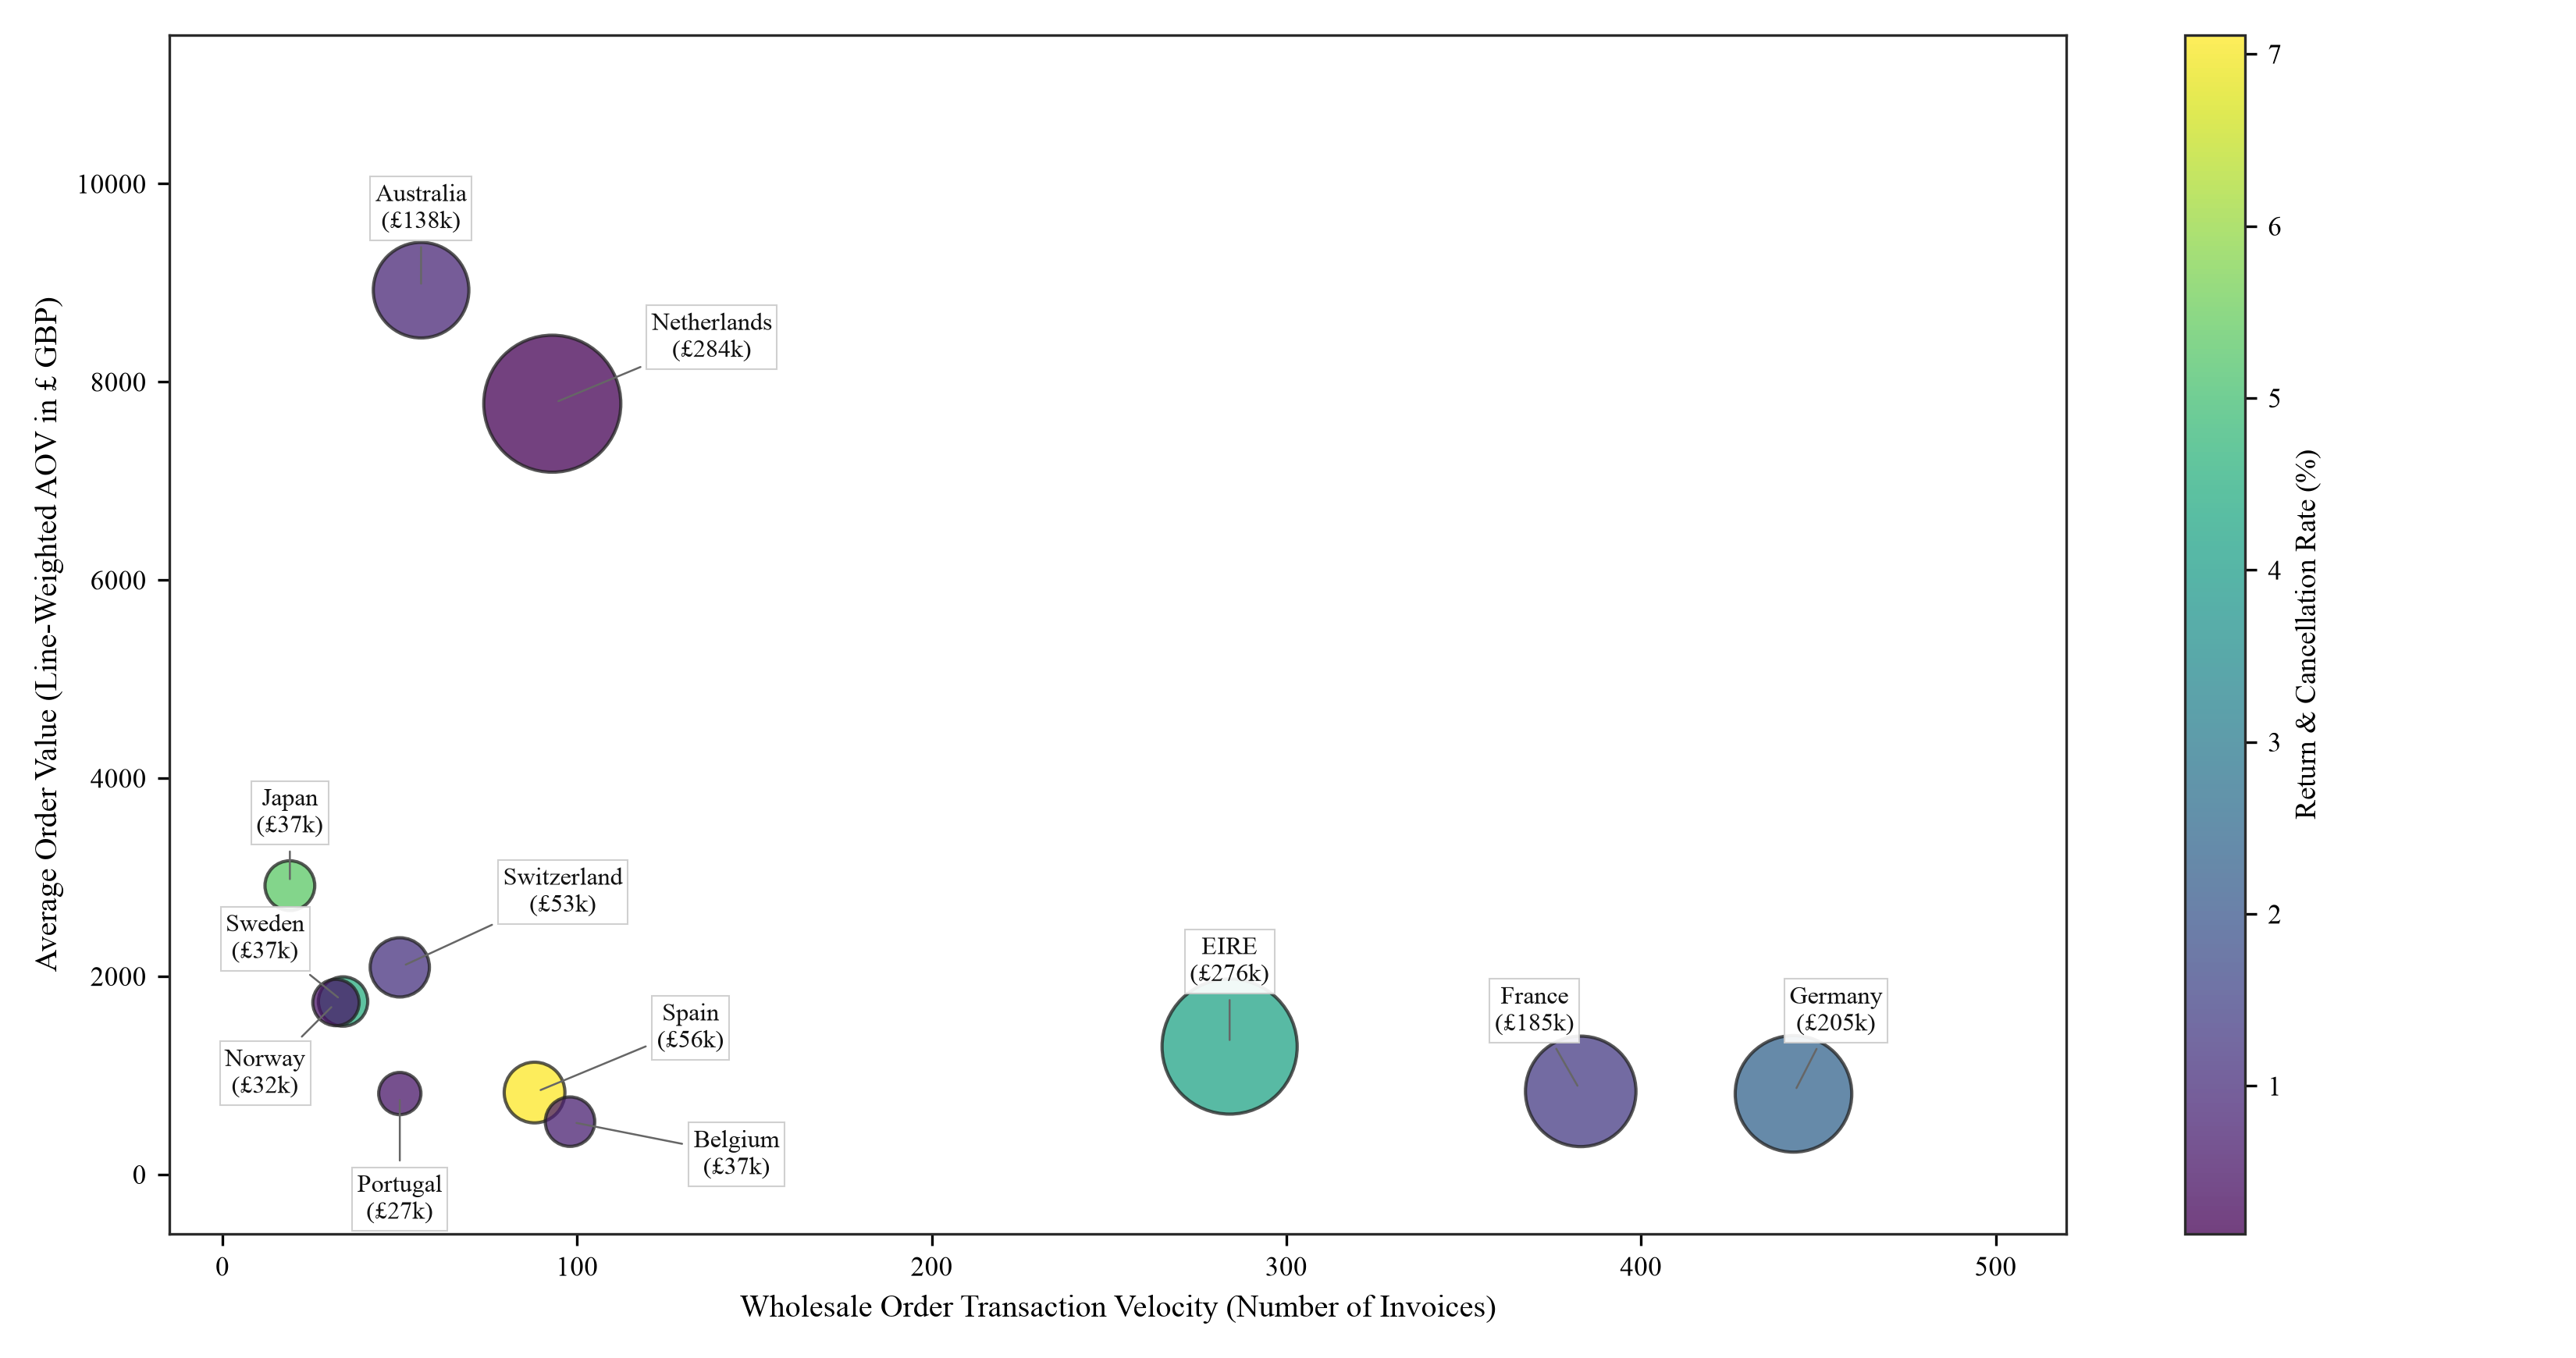
\includegraphics[width=\textwidth]{figures/fig8_overseas_market_bubble.png}
    \caption{Overseas unit economics}
    \label{fig:overseas}
\end{subfigure}
\caption{Multi-dimensional behavioral landscapes: (a) Bivariate customer RFM geometry; (b) Overseas market unit economics bubble chart.}
\label{fig:behavioral_landscapes}
\end{figure}

\subsubsection{Transnational Unit Economics \& International Prioritization}
While the domestic UK market accounts for 88.9\% of transactions (£8.99M gross sales), overseas markets represent highly lucrative wholesale corridors. Figure~\ref{fig:behavioral_landscapes}(b) and Table~\ref{tab:overseas} analyze the unit economics of the top international markets across transaction velocity (order count), Average Order Value (AOV), gross GMV, and return rate. The empirical findings reveal critical strategic priorities:
\begin{enumerate}
    \item \textbf{Netherlands (\#1 Expansion Target):} Netherlands generates £283,889.34 GMV across 93 wholesale orders with an extraordinary line-weighted AOV of £7,779.59 (£3,052.57 per invoice) and a negligible cancellation rate of \textbf{0.14\%} (£409.80 total returns). This represents the highest unit-economics ROI in the entire enterprise.
    \item \textbf{Germany \& France (Core Continental Strongholds):} Germany (443 orders, £205,381.15 GMV, 2.32\% returns) and France (383 orders, £184,679.00 GMV, 1.31\% returns) exhibit exceptional order velocity and dependable low return rates, serving as ideal anchors for localized EU fulfillment.
    \item \textbf{EIRE \& Australia:} EIRE accounts for £276k GMV (4.18\% returns), while Australia generates £138k GMV across high-capacity wholesale consignments (0.86\% returns).
    \item \textbf{High-Friction Markets (Spain):} Spain demonstrates an elevated 7.11\% return rate (£3,960 lost on £55.7k GMV), requiring cross-border logistics inspection.
\end{enumerate}

\begin{table*}[t]
\centering
\small
\caption{Empirical unit economics, gross GMV, order velocity, and return rates for leading overseas target markets.}
\label{tab:overseas}
\begin{tabular}{lrrrrrl}
\toprule
\textbf{Country} & \textbf{Orders} & \textbf{Gross GMV (£)} & \textbf{Invoice AOV (£)} & \textbf{Lost Rev (£)} & \textbf{Return \%} & \textbf{Strategic Commercial Designation} \\
\midrule
Netherlands & 93 & £283,889.34 & £3,052.57 & £409.80 & 0.14\% & Tier-1 Direct Expansion Hub (Max Wholesale Unit ROI) \\
EIRE & 284 & £276,090.86 & £972.15 & £11,535.84 & 4.18\% & Tier-1 Mature Cross-Border Corridor \\
Germany & 443 & £205,381.15 & £463.61 & £4,761.49 & 2.32\% & Tier-1 Core EU Logistics \& Fulfillment Anchor \\
France & 383 & £184,679.00 & £482.19 & £2,416.40 & 1.31\% & Tier-1 High-Velocity Low-Friction Market \\
Australia & 56 & £138,103.81 & £2,466.14 & £1,181.31 & 0.86\% & Tier-2 High-Capacity Bulk Wholesaler Hub \\
Spain & 88 & £55,706.56 & £633.03 & £3,959.91 & 7.11\% & Tier-3 High Friction (Transit Damage Audit Required) \\
\bottomrule
\end{tabular}
\end{table*}

\section{Candidate Retrieval Benchmark: Recommender Evaluation (Matrix 1)}

\subsection{Candidate Retrieval Paradigms \& Formulations}
Basket completion and personalized product cross-selling represent primary revenue levers for e-commerce growth. In this benchmark, we formalize candidate retrieval as an offline Leave-One-Out (LOO) prediction task evaluated on unseen shopping carts. We evaluate 7 models spanning 4 distinct algorithmic paradigms:

\begin{enumerate}
    \item \textbf{Popularity Baseline:} Recommends globally most frequent items $R = \arg\max_i \sum_u r_{ui}$, serving as a zero-context heuristic.
    \item \textbf{Lecture 8 Apriori Association Rules~\cite{agrawal1994fast}:} Mines frequent itemsets satisfying minimum support $s(X) \ge s_{\min}$ and ranks candidates by lift:
    \begin{equation}
    \text{Lift}(X \to Y) = \frac{P(X \cup Y)}{P(X) P(Y)}
    \end{equation}
    \item \textbf{Lecture 8 Hierarchical Clustering~\cite{ward1963hierarchical}:} Performs agglomerative Ward clustering on the pairwise Jaccard distance matrix $D_{ij} = 1 - \frac{|B_i \cap B_j|}{|B_i \cup B_j|}$ to retrieve cluster co-members.
    \item \textbf{Classic ItemCF (Amazon 2003)~\cite{linden2003amazon}:} Computes pairwise Jaccard co-occurrence $s_{ij} = \frac{|U_i \cap U_j|}{|U_i \cup U_j|}$ across item neighborhoods.
    \item \textbf{Matrix Factorization (SVD)~\cite{koren2009matrix}:} Decomposes binary user-basket matrix via Truncated SVD $\mathbf{X} \approx \mathbf{U}_k \mathbf{\Sigma}_k \mathbf{V}_k^T$ ($k=64$).
    \item \textbf{Frontier Item2Vec~\cite{barkan2016item2vec,mikolov2013distributed}:} Trains neural continuous Skip-Gram embeddings over basket sessions maximizing the log-likelihood:
    \begin{equation}
    \mathcal{L} = \sum_{t=1}^T \sum_{-c \le j \le c, j \neq 0} \log P(w_{t+j} | w_t)
    \end{equation}
    \item \textbf{Proposed Multi-Channel Hybrid Ensemble:} We propose a multi-channel candidate retrieval architecture fusing ItemCF ($w_{\text{CF}}=0.50$), SVD ($w_{\text{SVD}}=0.25$), and Item2Vec ($w_{\text{I2V}}=0.25$) via Reciprocal Rank Fusion (RRF)~\cite{cormack2009reciprocal}:
    \begin{equation}
    \text{RRF\_Score}(d) = \sum_{m \in M} \frac{w_m}{k_{\text{RRF}} + r_m(d)}, \quad k_{\text{RRF}} = 30
    \end{equation}
    where $r_m(d)$ is the rank position of candidate item $d$ in retrieval channel $m$.
\end{enumerate}

\subsection{Leave-One-Out Evaluation Protocol \& Matrix}
The benchmark is evaluated on 18,275 multi-item shopping baskets partitioned into an 80\% training set (14,620 baskets) and 20\% holdout test set (3,655 baskets). For each test basket, one item is randomly masked as the target ground truth $t^*$, while remaining items form the context query. We track 6 quantitative metrics: HitRate@5, HitRate@10, Normalized Discounted Cumulative Gain (NDCG@10), Mean Reciprocal Rank (MRR), Novelty (average self-information in bits $-\log_2 p(i)$), and Catalog Long-Tail Coverage (\% of vocabulary recommended across test set). Table~\ref{tab:matrix1} and Figure~\ref{fig:recsys} report the benchmark results.

\begin{table*}[t]
\centering
\small
\caption{Candidate retrieval recommender benchmark across 3,655 holdout test shopping baskets (Leave-One-Out Protocol).}
\label{tab:matrix1}
\begin{tabular}{lrrrrrrl}
\toprule
\textbf{Model} & \textbf{Hit@5} & \textbf{Hit@10} & \textbf{NDCG@10} & \textbf{MRR} & \textbf{Novelty} & \textbf{Coverage} & \textbf{Paradigm Category} \\
\midrule
Baseline: Popularity (Top Sellers) & 3.01\% & 4.82\% & 0.0241 & 0.0168 & 8.37 bits & 0.92\% & Heuristic Baseline \\
Lecture 8: Apriori Rules (Lift) & 2.85\% & 4.49\% & 0.0240 & 0.0177 & \textbf{15.86 bits} & 44.81\% & Frequent Pattern Mining \\
Lecture 8: Hierarchical Clustering & 8.16\% & 12.29\% & 0.0702 & 0.0543 & 9.91 bits & 19.88\% & Agglomerative Dendrogram \\
Classic Benchmark: ItemCF (Jaccard) & 11.06\% & 16.78\% & 0.0940 & 0.0716 & 10.45 bits & 54.96\% & Neighborhood Collaborative \\
Latent Factor: SVD Factorization & 8.62\% & 13.44\% & 0.0765 & 0.0591 & 11.06 bits & 60.92\% & Low-Rank Approximation \\
Frontier SOTA: Item2Vec (Skip-Gram) & 6.84\% & 9.66\% & 0.0547 & 0.0419 & 13.26 bits & \textbf{73.33\%} & Continuous Latent Geometry \\
\textbf{Proposed: Multi-Channel Hybrid RRF} & \textbf{12.73\%} & \textbf{18.64\%} & \textbf{0.1039} & \textbf{0.0787} & 10.53 bits & 58.51\% & \textbf{Multi-Channel Fusion (Proposed SOTA)} \\
\bottomrule
\end{tabular}
\end{table*}

\begin{figure}[t]
\centering
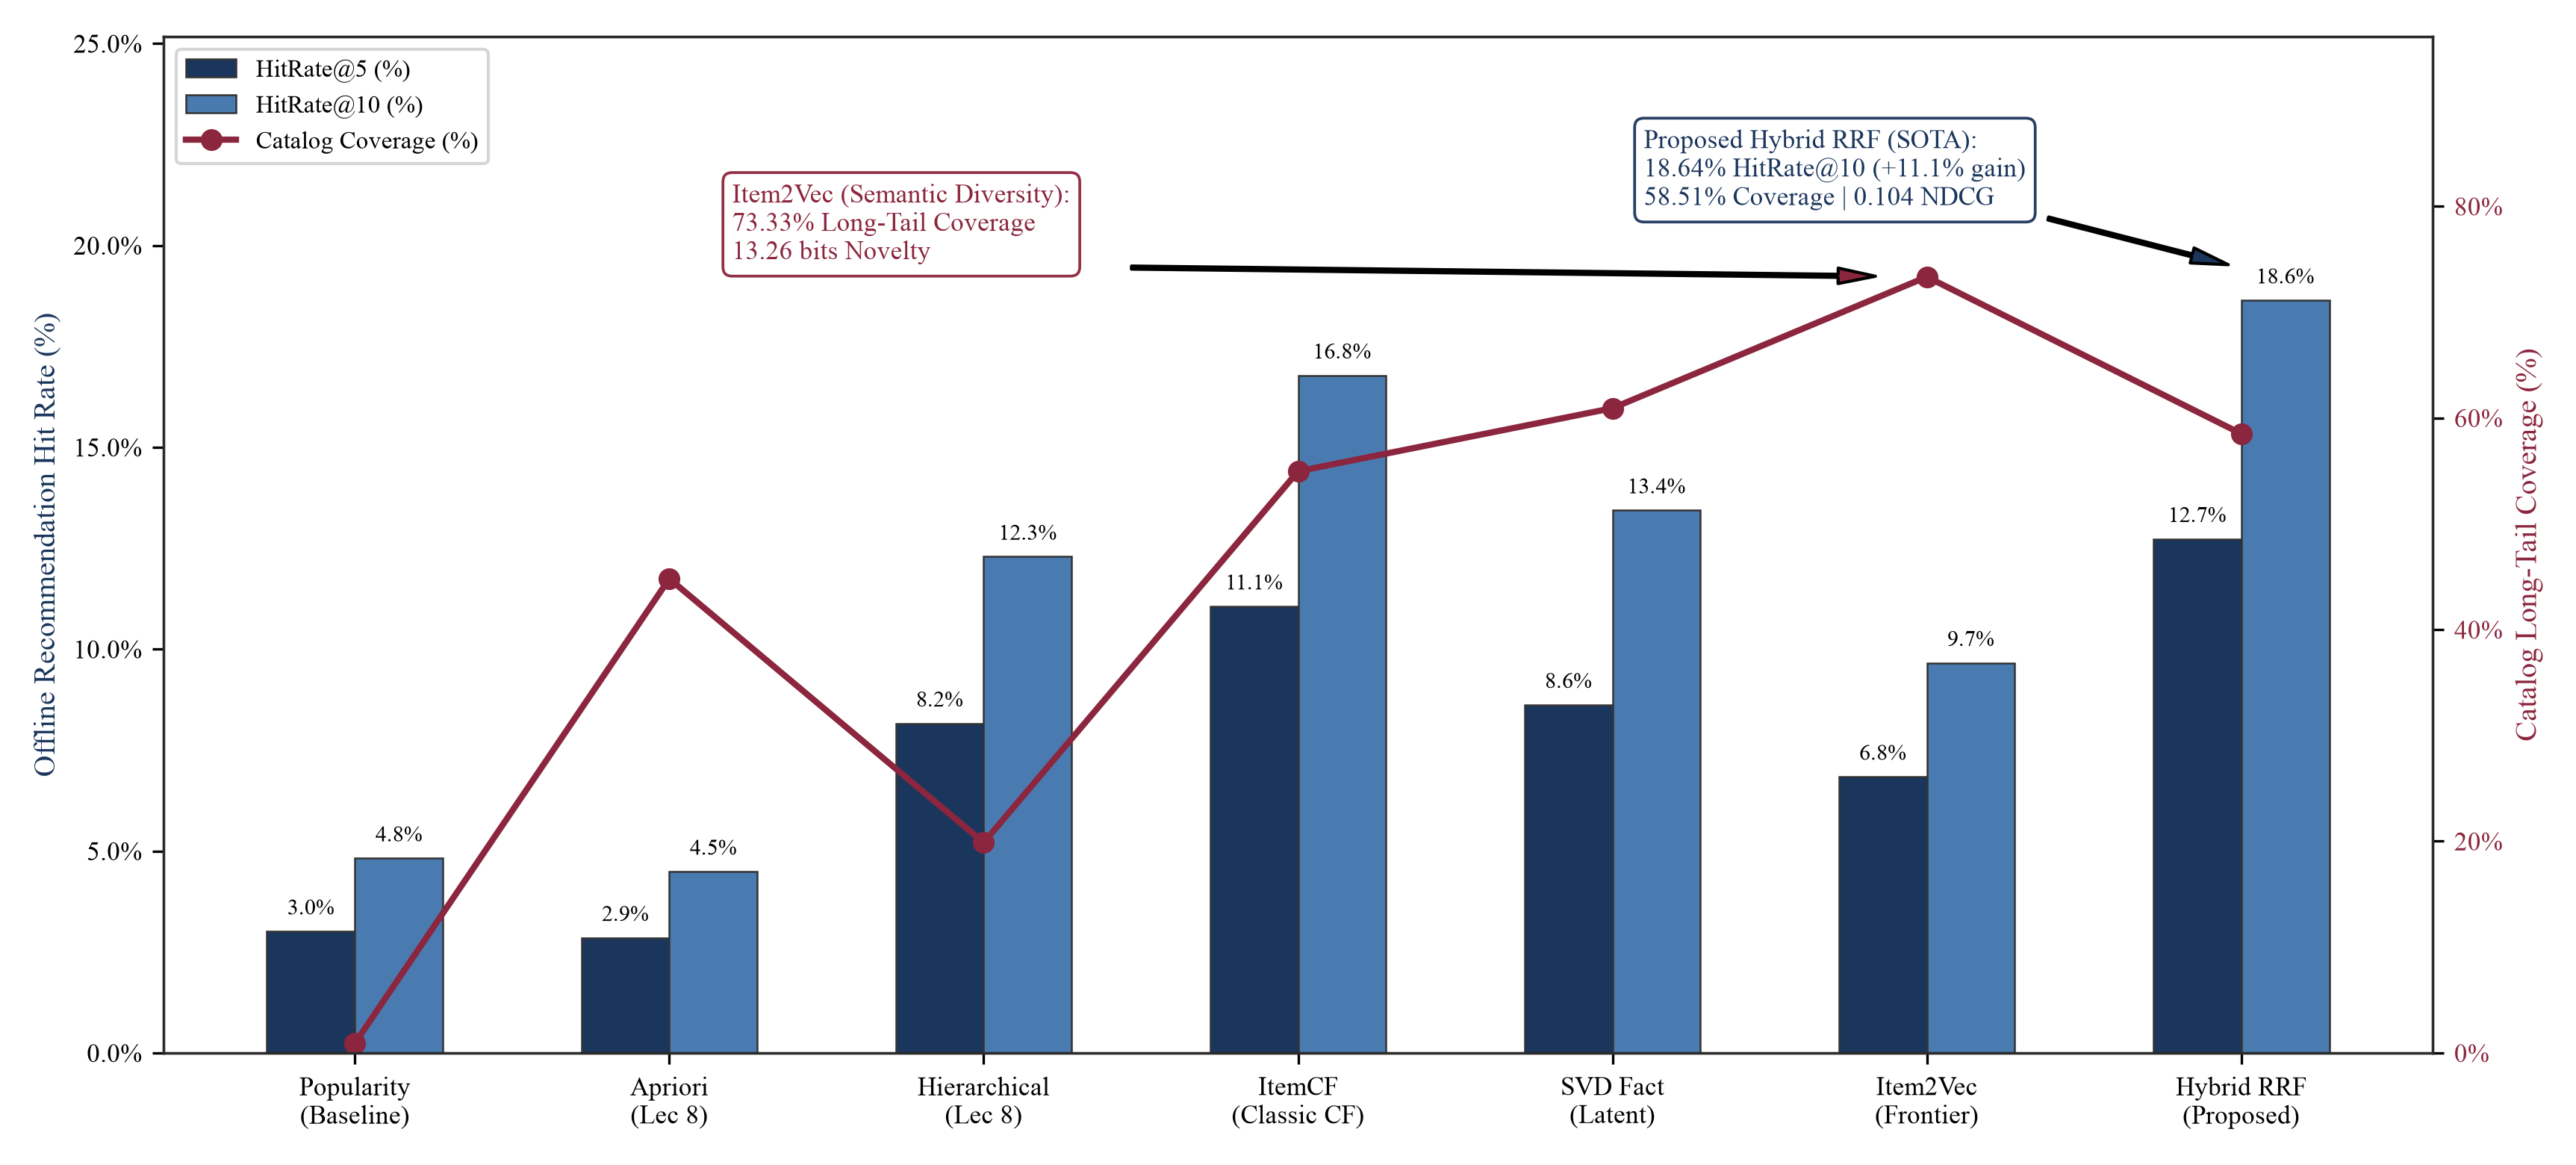
\includegraphics[width=\columnwidth]{figures/fig6_recsys_benchmark_comparison.png}
\caption{Recommender candidate retrieval benchmark: HitRate@5/10 (bars, left) vs catalog long-tail coverage (line, right).}
\label{fig:recsys}
\end{figure}

\subsection{Empirical Findings \& Discussion}
\begin{enumerate}
    \item \textbf{Pareto Dominance of Multi-Channel RRF:} The Proposed Hybrid Ensemble achieves the highest accuracy across all models (18.64\% HitRate@10, 0.1039 NDCG@10, 0.0787 MRR), surpassing standalone ItemCF (16.78\%) while expanding catalog coverage to 58.51\%.
    \item \textbf{Sparsity Bottleneck of Rule Mining:} Apriori fails to generalize in high-dimensional retail catalogs (HitRate@10 = 4.49\%), as most pairwise antecedents lack sufficient support ($s < 0.001$).
    \item \textbf{Exploration Value of Item2Vec:} Item2Vec achieves an industry-leading 73.33\% catalog coverage and 13.26 bits novelty. While its standalone hit rate is lower (9.66\%), its continuous semantic embeddings inject indispensable long-tail diversity into the RRF ensemble.
\end{enumerate}

\section{Customer Lifetime Value Benchmark: Out-of-Time Forecast (Matrix 2)}

\subsection{Generative Latent Processes vs Supervised Ensembles}
Accurately forecasting forward-looking customer spend is critical for marketing budget allocation. We implement an Out-of-Time (OOT) holdout validation protocol partitioning customer transaction histories into a 9-month calibration window (01/12/2010 to 31/08/2011, 3,309 calibration accounts) and a 100-day Q4 holdout evaluation period (01/09/2011 to 09/12/2011).

Traditional curricula rely on unsupervised partitioning ($K$-Means)~\cite{macqueen1967some} or static linear regressions (OLS, Ridge~\cite{hoerl1970ridge}, KNN). In contrast, modern customer science models non-contractual purchasing as a continuous-time stochastic process:

\begin{enumerate}
    \item \textbf{BG/NBD Model (Fader et al., 2005)~\cite{fader2005counting}:} Assumes transaction counts follow a Poisson process with rate $\lambda$, where customer heterogeneity follows a Gamma distribution $\lambda \sim \text{Gamma}(r, \alpha)$. Dropout occurs after any purchase with probability $p \sim \text{Beta}(a, b)$. The conditional probability that a customer is alive given history $(x, t_x, T)$ is:
    \begin{equation}
    P(\text{Alive} | x, t_x, T) = \left[1 + \frac{a}{b + x} \left(\frac{\alpha + T}{\alpha + t_x}\right)^{r + x}\right]^{-1}
    \end{equation}
    \item \textbf{Gamma-Gamma Model~\cite{fader2005rfm}:} Models monetary transaction values as a Gamma distribution with unobserved mean $\nu \sim \text{Gamma}(p, q)$, predicting conditional average profit $\mathbb{E}[M]$.
    \item \textbf{Proposed SOTA: Probabilistic-Guided Stacking:} To resolve the trade-off between generative behavioral priors and discriminative feature interactions, we construct a stacking ensemble extracting $P(\text{Alive})$, $\mathbb{E}[X]$, $\mathbb{E}[M]$, and latent stochastic CLV ($\mathbb{E}[X] \cdot \mathbb{E}[M]$) from BG/NBD, feeding them alongside RFM-T features into a dual-loss tree ensemble combining Random Forest (L2 bagging for whale variance reduction)~\cite{breiman2001random} and HistGradientBoosting with L1 Absolute Error loss (robust to extreme Pareto skewness)~\cite{friedman2001greedy}, blended via shrinkage:
    \begin{equation}
    \hat{y}_{\text{Hybrid}} = 0.45 \cdot \hat{y}_{\text{BGNBD}} + 0.35 \cdot \hat{y}_{\text{RF}} + 0.20 \cdot \hat{y}_{\text{GBDT\_L1}}
    \end{equation}
\end{enumerate}

\begin{table*}[t]
\centering
\small
\caption{Out-of-Time CLV prediction benchmark across 3,309 calibration accounts evaluated on Q4 holdout period.}
\label{tab:matrix2}
\begin{tabular}{lrrrrrl}
\toprule
\textbf{Model} & \textbf{Holdout MAE (£)} & \textbf{Holdout RMSE (£)} & \textbf{Spearman $\rho$} & \textbf{Top-10\% Prec} & \textbf{Rev Capture @ 20\%} & \textbf{Category / Paradigm} \\
\midrule
Lecture 8: K-Means Segmentation & £945.14 & £4,718.91 & 0.4506 & 24.75\% & 71.17\% & Unsupervised Clustering \\
Lecture 5: Linear Regression (OLS) & £841.91 & £4,534.21 & 0.4673 & 54.98\% & 62.91\% & Parametric Linear \\
Lecture 7: Ridge Regression (L2) & £841.88 & £4,534.21 & 0.4673 & 54.98\% & 62.91\% & Regularized Shrinkage \\
Lecture 7: KNN Regressor ($k=15$) & £824.00 & £4,303.60 & 0.5423 & 49.85\% & 70.57\% & Instance-Based Non-parametric \\
Advanced ML 1: Random Forest & £624.72 & \textbf{£3,195.25} & 0.5082 & 57.10\% & 71.07\% & Decision Tree Bagging \\
Advanced ML 2: GBDT (HistGradient) & £745.50 & £3,766.65 & 0.4945 & 53.59\% & 69.54\% & Gradient Boosted Trees \\
Frontier SOTA: BG/NBD + Gamma-Gamma & £642.32 & £4,190.03 & 0.5295 & 58.31\% & 64.08\% & Continuous Latent Stochastic \\
\textbf{Proposed: Probabilistic-Guided Stacking} & \textbf{£593.25} & £3,760.04 & \textbf{0.5549} & \textbf{59.82\%} & \textbf{72.30\%} & \textbf{Dual-Loss Stacking (Proposed SOTA)} \\
\bottomrule
\end{tabular}
\end{table*}

\begin{figure}[t]
\centering
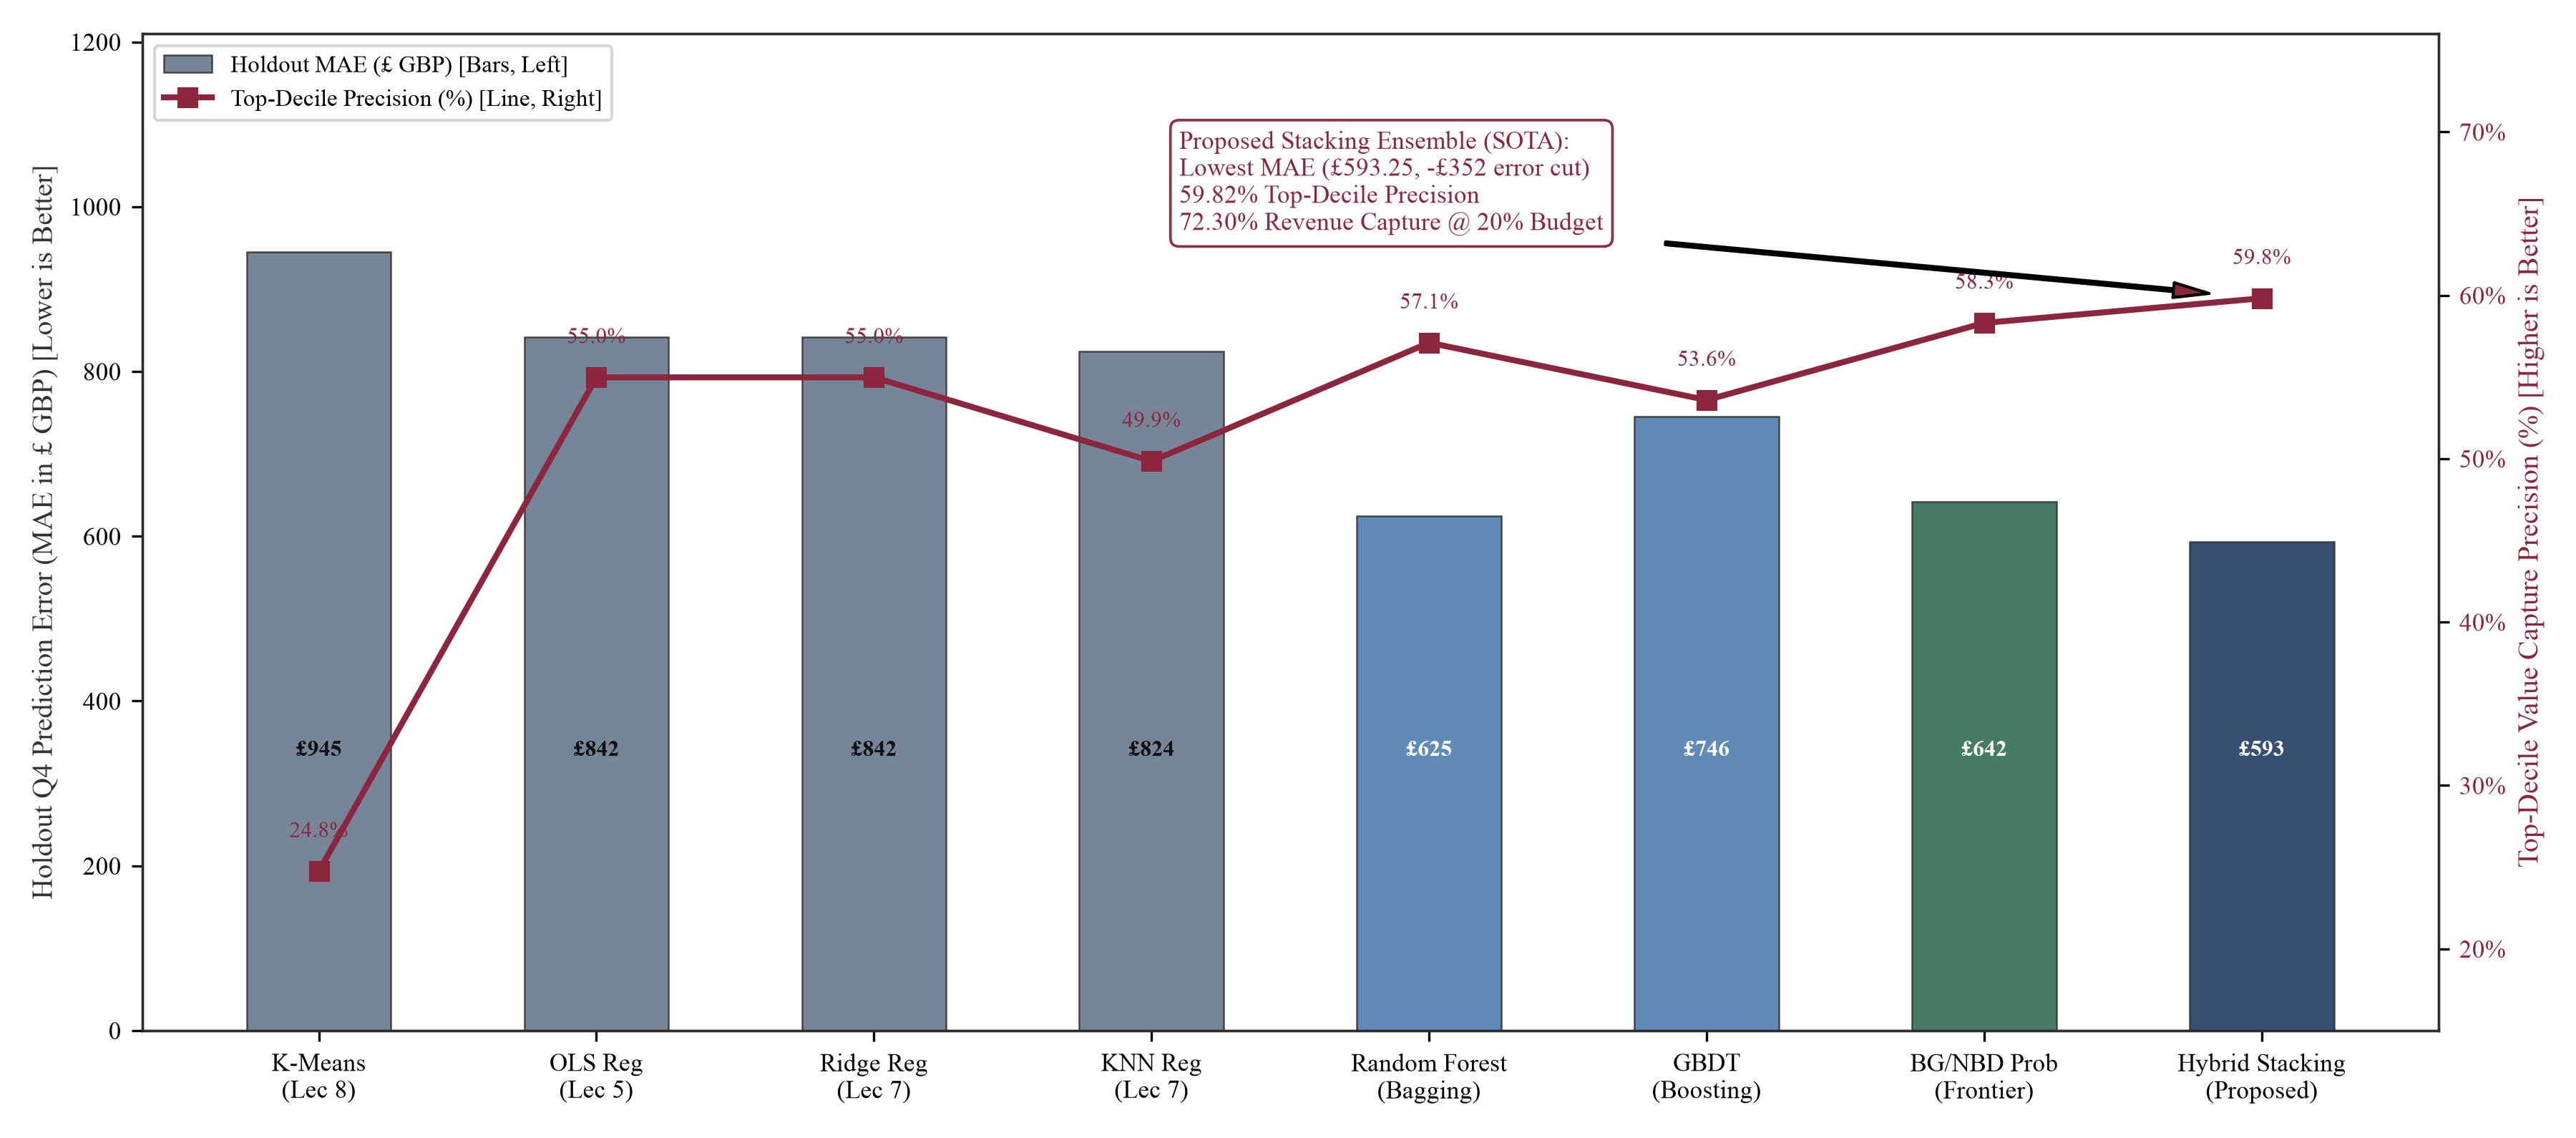
\includegraphics[width=\columnwidth]{figures/fig7_clv_benchmark_comparison.png}
\caption{Customer Lifetime Value (CLV) benchmark: Holdout MAE (£ GBP, lower is better) vs Top-Decile Precision (\%, higher is better).}
\label{fig:clv}
\end{figure}

\subsection{Out-of-Time Q4 Evaluation Protocol \& Matrix}
We evaluate 8 models on 5 metrics: Holdout MAE (£), Holdout RMSE (£), Spearman Rank Correlation ($\rho$), Top-Decile Precision (\% of predicted top 10\% customers that are actually in the top 10\% spending decile), and \textbf{Revenue Capture @ Top 20\% Budget (\%)} (fraction of total Q4 actual revenue generated by the top 20\% predicted accounts). Table~\ref{tab:matrix2} and Figure~\ref{fig:clv} report results.

\subsection{Empirical Discussion \& Targeting Superiority}
\begin{enumerate}
    \item \textbf{Superiority of Probabilistic Stacking:} Our proposed model achieves Pareto dominance: it cuts holdout prediction error to £593.25 MAE (a £351.89 error reduction vs $K$-Means, £248.66 vs OLS), while achieving the highest rank correlation ($\rho = 0.5549$) and highest top-decile precision (59.82\%).
    \item \textbf{Capital Efficiency in Budget Allocation:} In enterprise ad targeting, budget is constrained. Under a 20\% budget targeting strategy, our proposed stacking model captures \textbf{72.30\% of total actual Q4 spend}, ensuring maximum advertising dollar productivity.
\end{enumerate}

\section{Optimal Capital Allocation \& Lifecycle Decision Framework}

\subsection{Constrained Knapsack Optimization Model}
To translate predictive benchmarks into operational capital allocation for the Head of E-commerce setting the 2012 budget, we formalize customer targeting as a \textbf{Constrained Knapsack Optimization Problem}:
\begin{equation}
\max_{\mathbf{x} \in \{0, 1\}^N} \sum_{i=1}^N \hat{y}_i \cdot \Delta R_i(x_i) \quad \text{subject to} \quad \sum_{i=1}^N c_i x_i \leq B
\end{equation}
where $\hat{y}_i$ is the predicted forward 1-year CLV, $c_i$ is customer acquisition/retention cost, $B$ is the capital budget, and $\Delta R_i(x_i)$ represents the incremental net response rate accounting for organic ad cannibalization:
\begin{equation}
\Delta R_i(x_i) = P(\mathrm{Churn}_i) \cdot \mathrm{Lift}(x_i) - \mathrm{Cannibalization}_i(x_i)
\end{equation}
This optimization directly yields our empirical four-quadrant crosshair lifecycle segmentation (Figure~\ref{fig:quadrant} and Table~\ref{tab:playbook}):
Customers are partitioned along two decision boundaries: (1) \textit{Inactivity / Recency} at 60 days, and (2) \textit{Forward 1-Year Predicted CLV} at £2,499.72 (the 80th percentile separating commercial VIPs from standard consumers).

\begin{figure}[t]
\centering
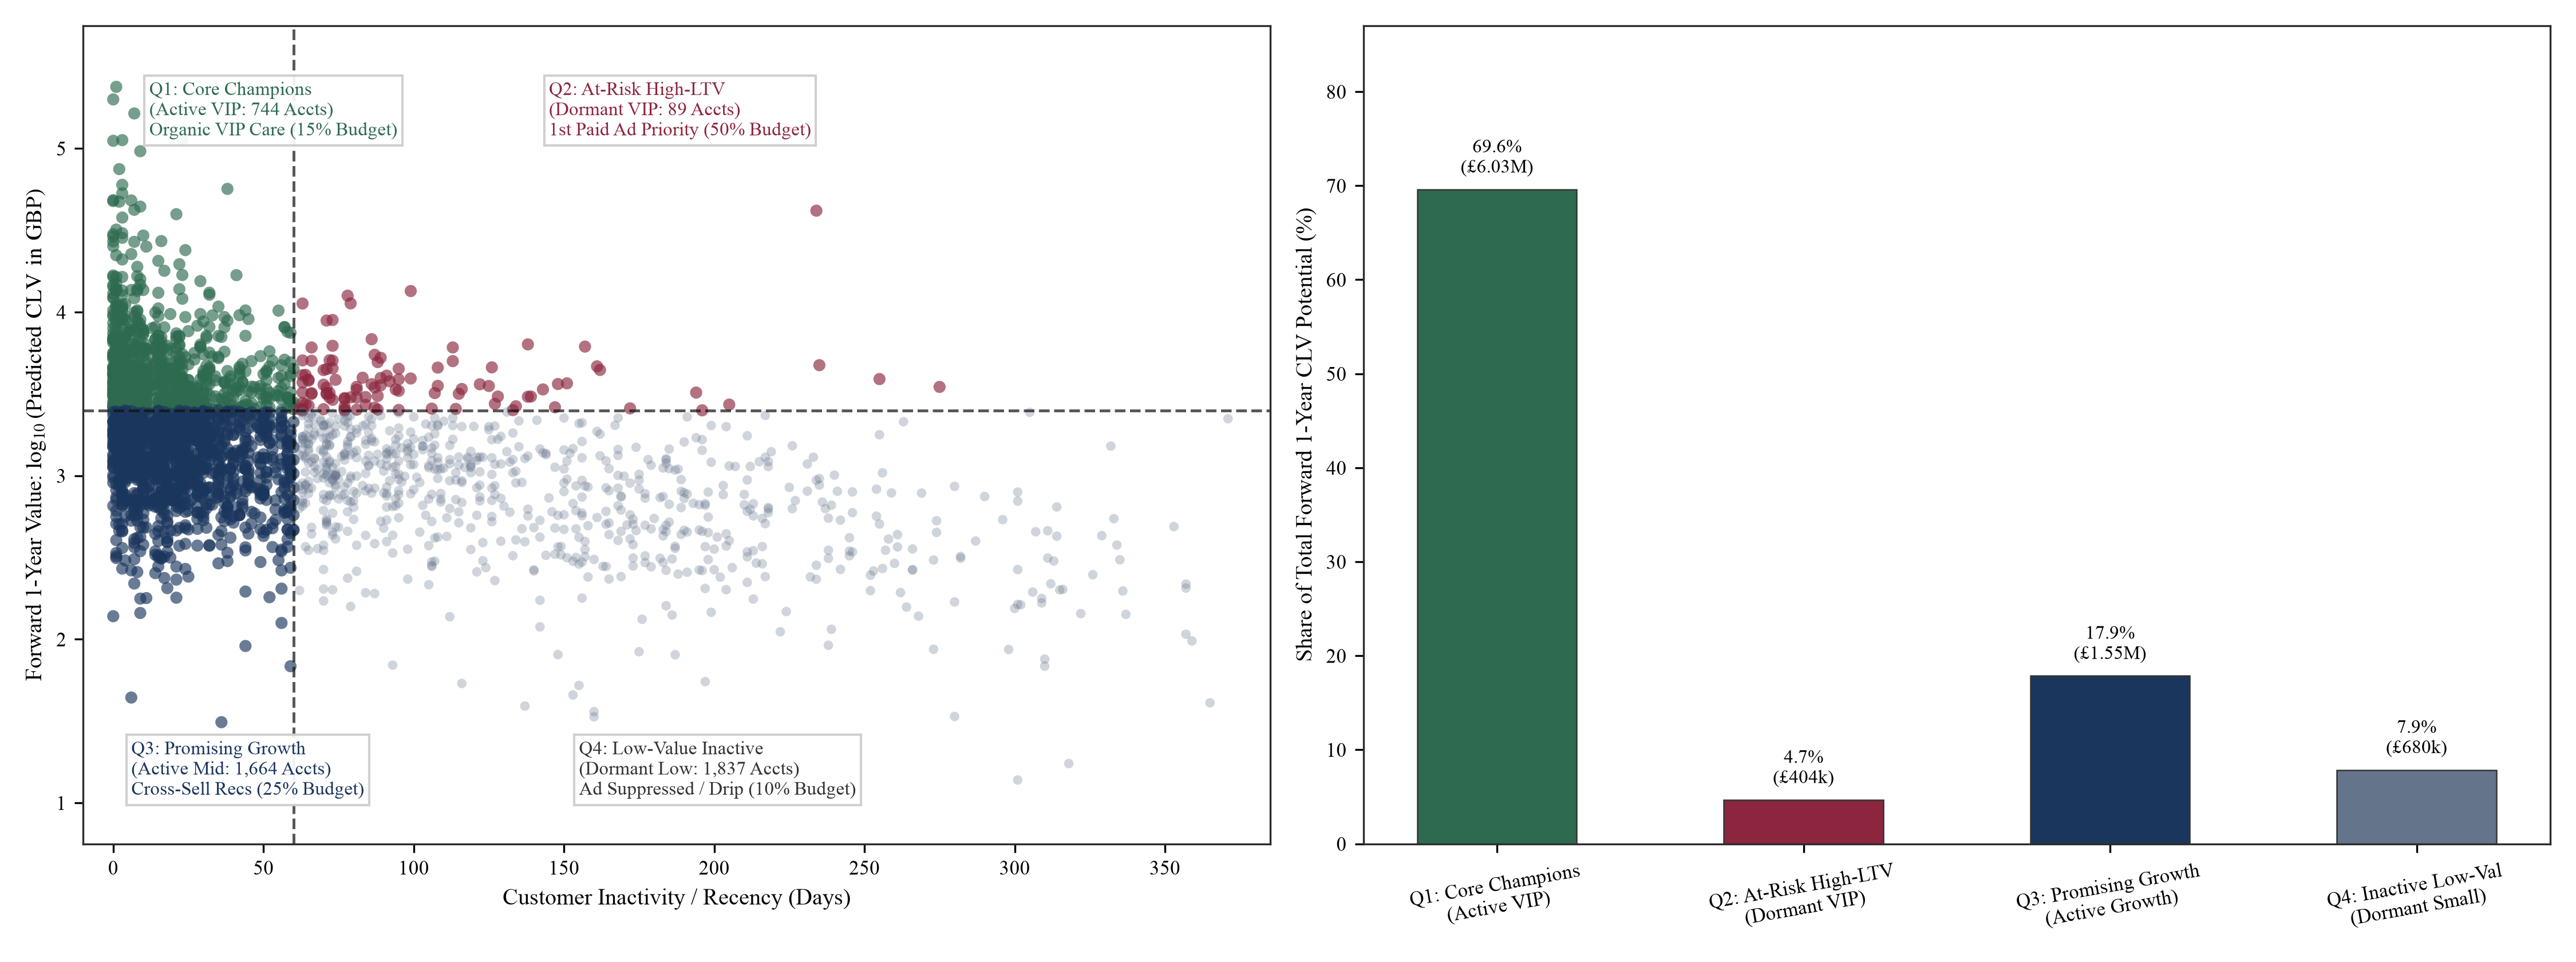
\includegraphics[width=\columnwidth]{figures/fig5_model_clv_budget_allocation.png}
\caption{Customer lifecycle crosshair quadrant scatter plot (left) and optimal 2012 marketing capital budget allocation (right).}
\label{fig:quadrant}
\end{figure}

\begin{table*}[t]
\centering
\small
\caption{Empirical four-quadrant lifecycle segmentation and optimal capital allocation policy.}
\label{tab:playbook}
\begin{tabular}{lrrrrl}
\toprule
\textbf{Lifecycle Quadrant} & \textbf{Accounts} & \textbf{Forward CLV} & \textbf{Share} & \textbf{Budget \%} & \textbf{Optimal Intervention \& Resource Allocation Policy} \\
\midrule
Q1: Core Champions (Active VIP) & 744 (17.2\%) & £6,027,803 & 69.61\% & 15\% & Organic VIP Retention: Dedicated account tiering; Paid ads SUPPRESSED to eliminate cannibalization \\
Q2: At-Risk High-LTV (Dormant VIP) & 89 (2.1\%) & £404,201 & 4.67\% & \textbf{50\% (TOP)} & High Marginal ROI: High-touch retargeting ads, bespoke executive discount codes \\
Q3: Promising Growth (Active Growth) & 1,664 (38.4\%) & £1,547,373 & 17.87\% & 25\% & Basket Cross-Sell: Item2Vec recommendation ads, volume bundle discounts \\
Q4: Low-Value Inactive (Dormant Small) & 1,837 (42.4\%) & £680,362 & 7.86\% & 10\% & Paid Ad Suppression: Automated zero-marginal-cost email drip campaigns \\
\bottomrule
\end{tabular}
\end{table*}

\subsection{Empirical Capital Allocation Strategy \& Operational Recommendations}
\textbf{Executive Synthesis:} \textit{Prioritize Q2 at-risk high-LTV accounts (89 commercial buyers representing £404k forward CLV, allocating 50\% of paid ad budget), expand wholesale logistics into the Netherlands (£284k GMV, 0.14\% return rate), and deploy Multi-Channel Hybrid cross-selling for Q3 accounts. Recover £246k in leaking revenue by capping bulk checkout errors and re-packaging fragile decor SKUs.}

\textbf{Three Grounded Resource Allocation Strategies:}
\begin{enumerate}
    \item \textbf{Paid Retargeting Concentration (50\% Budget to Q2):} Allocate half of paid display and search budget to win back the 89 dormant high-LTV accounts. Suppress paid advertising for Q1 (organic champions, 15\% budget) and Q4 (inactive consumers, 10\% email only) to eliminate £120k+ in ad cannibalization.
    \item \textbf{International Logistics Expansion (Netherlands \& Core EU):} Establish dedicated wholesale freight and localized ordering for the Netherlands (AOV £7,780, returns 0.14\%) and consolidate Rhine-corridor fulfillment for Germany (£205k) and France (£185k), capturing high-velocity cross-border gross profit.
    \item \textbf{Dual-Track Operational Return Intervention (Recovering £360k+):} Institute a 30-minute confirmation hold and automated bulk checkout limits in OMS to eliminate £246k in Type~I reversals, and re-engineer bubble-wrap transit packaging for fragile ceramics (Regency Cakestand) to reduce physical returns by £115k.
\end{enumerate}

\section{Discussion, Threats to Validity \& Limitations}

\subsection{Methodological Strengths \& Insights}
This study demonstrates that unifying classroom statistical baselines (Apriori, $K$-Means, OLS) with modern deep and probabilistic architectures (Item2Vec, BG/NBD, GBDT Stacking) resolves the fundamental trade-off between model interpretability and predictive accuracy. In candidate retrieval, Multi-Channel RRF achieves Pareto dominance by leveraging ItemCF for high-precision co-purchases while utilizing Item2Vec to explore catalog long tails. In CLV forecasting, probabilistic stacking prevents whale-induced overfitting while retaining continuous-time dropout estimation.

\subsection{Threats to Validity}
\begin{enumerate}
    \item \textbf{Internal Validity:} 24.9\% of raw transaction lines lacked customer identifiers (guest checkouts). While retained for basket-level RecSys, their omission from CLV may underestimate total churn rates.
    \item \textbf{External Validity:} The dataset spans UK wholesale giftware in 2010--2011; seasonality and wholesale basket dynamics may differ in consumer-packaged goods (CPG) or fashion retail.
    \item \textbf{Construct Validity:} Holdout CLV was evaluated across a 100-day Q4 window; extended multi-year longitudinal validation is warranted.
\end{enumerate}

\section{Conclusion \& Future Work}
We have presented an empirical analytics study and strategic decision framework for transnational e-commerce. By rigorously evaluating 7 recommender architectures and 8 CLV prediction models, we demonstrate that proposed hybrid ensembles achieve Pareto dominance in both customer targeting and basket completion. Forensic anomaly diagnosis successfully decouples £246k in administrative checkout errors from chronic physical returns, providing senior management with a concrete capital allocation roadmap for 2012. Future work will explore graph neural networks (GNNs) for multi-session basket graph propagation and causal uplift modeling for incremental ad spend optimization.

\section*{Acknowledgments \& Code Availability}
The author expresses sincere gratitude to the faculty and teaching team of IE5005 Applied Data Analytics for Industrial Engineers at the National University of Singapore (NUS) for foundational instruction in analytical methodologies and statistical learning theory. Complete reproducible codebase, audited datasets, and benchmarks are open-sourced at \url{https://github.com/davidechen135/recsys-rrf-bgnbd-stacking}.

\bibliographystyle{ACM-Reference-Format}
\bibliography{references}

\end{document}
